\documentclass{kupaper}
\usepackage{jtygm}%%%%%%%%%%%%%%%%%Font Warning対策%%%%%
\usepackage{float}
\usepackage[dvipdfmx]{graphicx}
\usepackage{multirow}

% プリアンブルに追加する

\includeonly{0,1,2,3,4,5,6,7,thanks}

\begin{document}



%序章
%#!platex --src-specials main.tex

\Title{触覚情報における加速度情報の取り扱いに関する検討} 
\Author{塩田 雅人}
\Date{2}{3}{5}

%学部の人は次のコメント行の%を外してください.
\senior  %この\seniorは\Synopsisの前であればどこに書いてもかまいません.

\Synopsis

\begin{Abstract}
%アブスト

近年,バーチャルリアリティ技術の発展とともに,ヘッドマウントディスプレイなどリッチな視聴覚情報が利用可能になりつつある.それにあわせ,触覚情報の実現も求められている.そのため,さまざまな触覚情報を提示する触覚ディスプレイが数多く研究されている.このような触覚ディスプレイのためのコンテンツとして,センサを用いて取得した触覚情報の分類が研究されつつある. その中でも加速度触覚情報は再現性に優れ, 触覚提示の研究へ発展が期待される. 
現在, 3軸加速度触覚情報の分類を行う際, 3軸を1軸の振動情報に統合し, 情報量を抑える手法がある. 
しかし3軸加速度情報から 1 軸の振動情報に次元削減を行う中で, 欠損した情報も再現性を考えると触覚情報において重要である可能性がある. 
本研究では,次元削減と正規化を行った3軸加速度触覚情報と, 無加工の 3 軸加速度触覚情報とをそれぞれ畳み込みニューラルネットワークを用いた機械学習で分類, 比較し,  分類精度の観点から触覚情報における 3 軸加速度情報の取扱いについて検討する. 
\end{Abstract}

%
% これより下は学部(卒業論文を書く人)には関係ありません. 
% 
% \title{English Titile}
% \author{Taro Kumamoto}
% \endate{February}{Day}{Year}

% \synopsis

% \begin{abstract}
% English
% \end{abstract}










% 修士論文の論文概要

% 修士論文については和文と英文の論文概要を次の要領で作成し,【5】のb.2として下
% さい。英文で本文を記述した場合も,論文概要は和文,英文の両方で作成することが望ま
% しい(詳細は指導教員の指示に従って下さい)。

% 1.論文概要(和文)の形式

%     a.修士論文と同じ体裁で作った表紙(図2)を付けます。ただし,題目と氏名の間
%     に,「論文概要」と書き添えて下さい。

%     b.研究の目的,論文全体のあらまし,各章の内容(簡単に),結論(やや詳し
%     く),得られた成果の意義を,この順序で3~5ページ程度にまとめて下さい。

% 2.論文概要(英文)の形式

%    a.修士論文と同じ体裁で作った表紙(図2)を英文で記載して付けます。ただし,題
%    目と氏名の間に, Synopsis と書き添えて下さい

%    b.研究の目的,論文全体のあらまし,結論を,100~300 語程度にまとめて下さい。


% 3.和文,英文ともに目次は付けないで下さい。また,原則として,図,表,式を用いな
% いで下さい。


\Maketitle
%\listoftables
%\listobfigures

%\setcounter{chapter}{20}

% 目次  (LaTeX の処理を少くする目的で,最後に書いています)
\pagenumbering{roman}
\setcounter{page}{1}
\tableofcontents

%#!platex --src-specials main.tex

\chapter{はじめに}
\pagenumbering{arabic}     % 絶対必要です.最初の章にのみ記述します.
%プレ 羅列のみ
\section{研究背景と目的}
モバイルデバイスの発達により我々はこれまでより多くの情報を取り入れるようになった. それに伴い情報と人が接する面であるインタフェースも重要性を増し, より人の感覚に沿うようなインタフェースが開発されている. 触覚情報を用いたインタフェースはヒトが知覚する触感覚の精密さとヒトの触感覚受容器官の自由度から注目されてきているが, 受容される触覚情報に基づいた触覚刺激を提示する, 触覚ディスプレイに関連する研究は研究分野としてはまだ新しく, 視覚における光学ディスプレイの情報提示手法に比べ確立に至っていない. そのため現在ヒトに受容される触覚情報を収集する研究が様々な手法で行われている \cite{abdulali2016data},\cite{strese2017content}.
手法により収集する触覚情報は異なっているが, そのなかでも触覚情報を加速度情報として収集する手法は再現性が高く, 多数の関連研究が存在する
\cite{kuchenbecker2010verrotouch},\cite{romano2011creating}. 
またこれらの研究の多くは触覚ディスプレイを用いた情報の適切な提示が可能となるように, 触覚情報の収集手法に加え, 得られた触覚情報の分類手法も検討している. 触覚情報の分類は主に機械学習によって行われており, 分類の精度向上が多くの研究の課題となっている. 

3軸加速度の触覚情報の取扱いについて, 多くの研究が用いている手法の一つに, 3軸加速度情報を1軸の振動情報に統合し, 情報量を抑える手法がある. これは皮膚構造中の振動刺激を知覚する受容器が振動方向の判別を得意としていないこと\cite{brisben1999detection}に加え触覚情報に基づいたテクスチャデータをレンダリングする際に, 計算コストを抑える事が可能であることに起因する. 
しかし3軸加速度情報から1軸の振動情報に次元削減を行う中で, 欠損した情報も再現性を考えると触覚情報において重要である可能性がある \cite{kurogi}.

本研究では, Agatsumaら\cite{agatsuma}によって得られた3軸加速度情報をもとに,次元削減などの信号処理をおこなった情報をそれぞれ畳み込みニューラルネットワーク (Convolutional Neural Network:  CNN \cite{lecun}) を用いた機械学習で分類し, 分類精度の観点から触覚情報における3軸加速度情報の取扱いについて検討する. 

本稿において触覚情報とはヒトの受容器官と触対象との間に生じた摩擦に起因する振動, 受容器によって受容される圧力, 熱等の情報をいう. 

\section{本論文の構成}
本章では, 本研究の背景と目的を述べた. 本稿の次章以降の構成を以下に示す. \ref{chap:haptic}章では, 本研究における前提知識と関連する先行研究を述べる. \ref{chap:method}章では, 本研究で用いる触覚情報の次元削減手法と機械学習手法について述べる. \ref{chap:exp}章では, 本研究の評価実験について述べる. \ref{chap:result}章では, 実施した評価実験に対しての得られた結果を掲載する. \ref{chap:cons}章では, 得られた結果に対しての考察を行う. \ref{chap:conc}章で結論を述べる.

% Local Variables:
% TeX-master: "main"
% mode: yatex
% End:















%#!platex --src-specials main.tex

\chapter{触覚の生理学的特徴と\\関連する先行研究}
\label{chap:haptic}
本章において,  触覚の生理学的特徴, 触覚情報の取り扱いに関する先行研究について概説する.  

\section{触覚の生理学的特徴}
\subsection{ヒトの皮膚構造}
ヒトの触覚は成人にして約\,1.6$-$1.8\,$\mathrm{m^2}$の面積と\,3$-$5\,$\mathrm{kg}$の重量を持つ最大の感覚器官であり,  身体で最も大きな器官で全体重のほぼ1/6の重さを占める.  皮膚は表皮, 真皮, 皮下組織の三層構造からなり, この皮膚内部に時空間的に異なる特性を持つ触覚受容器が固有の位置に分布している. 皮膚構造を以下の図\ref{fig:skin}に示す. 
\begin{figure}[H]
\begin{center}
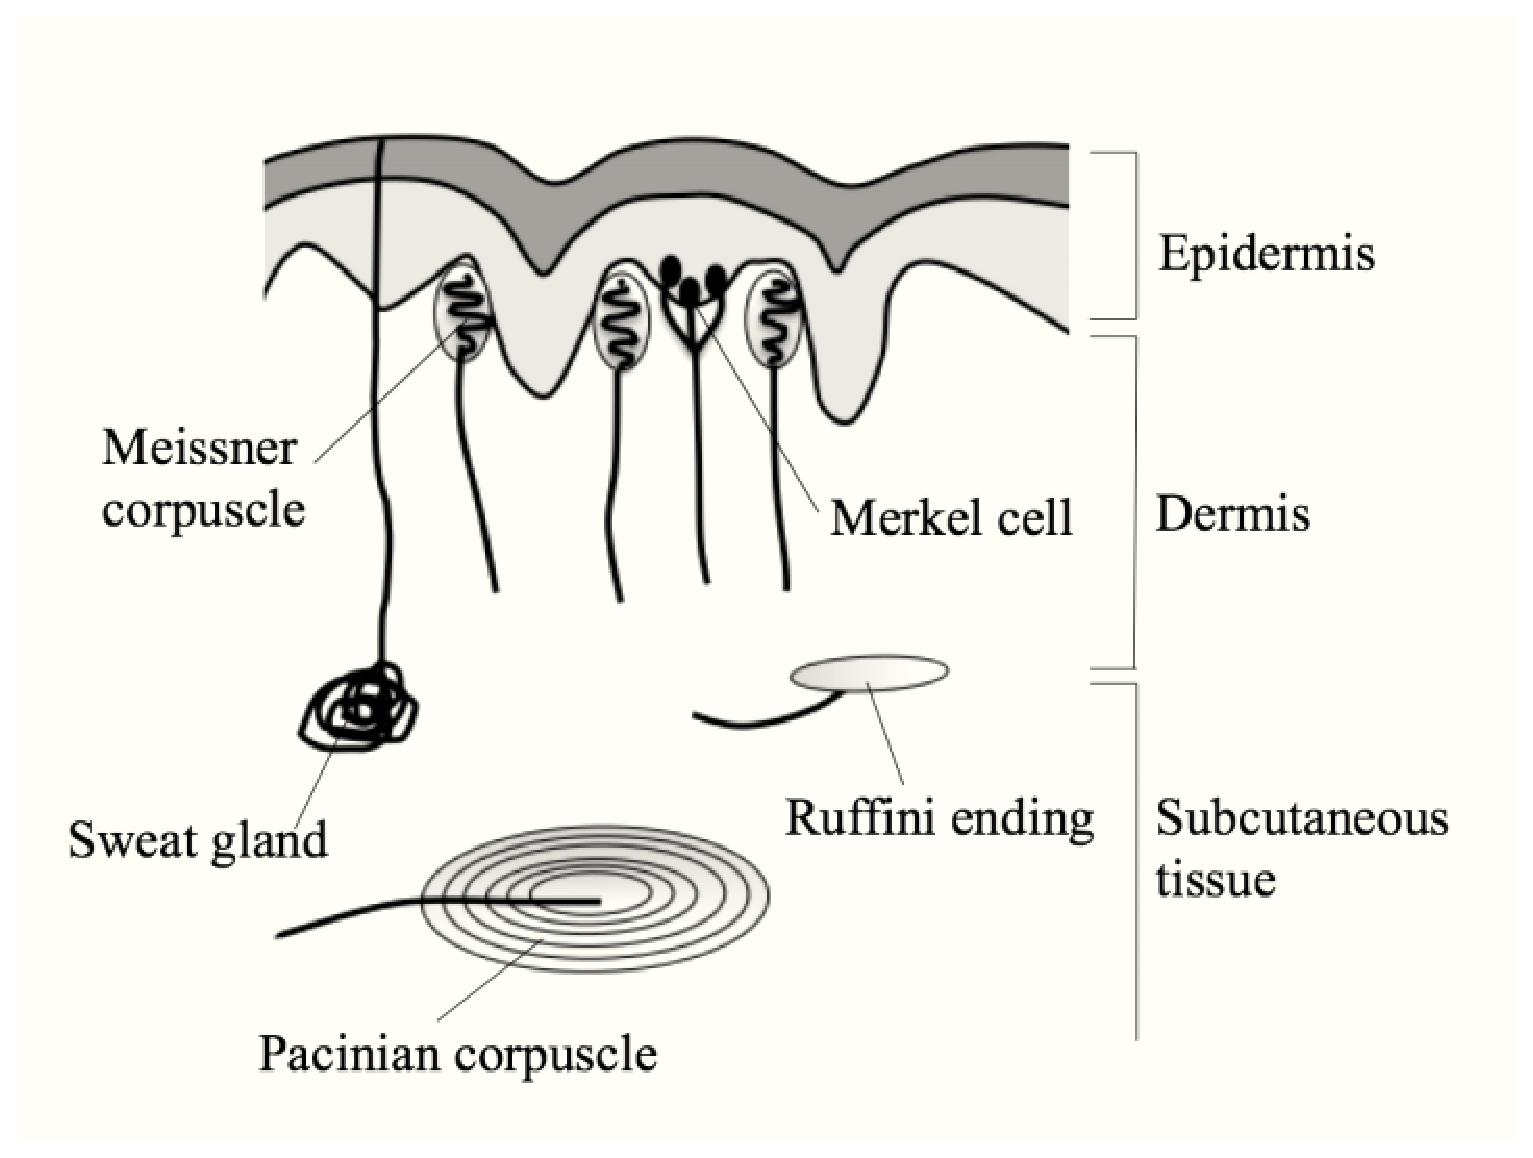
\includegraphics[width=8cm]{eps/skin_str.eps}
\caption{皮膚構造(\cite{mechanizm}より引用)}
\label{fig:skin}
\end{center}
\end{figure}

\subsection{触覚受容器}
無毛部皮膚に存在する触覚受容器において,  表皮の最深部に存在するメルケル小体 (Merkel discs), 真皮の最外層にあるマイスナー小体 (Meissner corpusde), 深層にあるパチニ小体 (Pacini corpuscle), ルフィニ終末 (Ruffini ending) の 4 つがよく知られている.
4つの受容器は応答の速さの違いから,  それぞれ\,Fast Adapting : FA,  \,Slow Adapting : SA に分類される \cite{1984438}.
また,  そこから触覚受容器の応答できる皮膚表面の範囲,  受容野の広さの違いからタイプ\rm\,I\,,  タイプ\rm\,II\,に分類される. 
これらの受容特性を表\ref{tab:Receptors}に示す \cite{前野隆司2000器用な手}.%\cite{2000772}.

\begin{table}[H]
 \caption{tactile receptors at glabrous skin}
 \label{tab:Receptors}
 \begin{center}
 \scalebox{0.8}{
\begin{tabular}{cllll}
\hline
Receptors          & type                                                     & receptive field & adaptation rate & size                                                              \\ \hline
Meissner corpuscle & FA\rm\,I\,  & small           & fast            & $L = 20-150\, \mathrm{\mu m},\, D = 40-70\, \mathrm{\mu m}$ \\
Merkel discs       & SA\rm\,I\,  & small           & slow            & $D = 7\, \mathrm{\mu m},\,T = 1\, \mathrm{\mu m}$           \\
Pacinian corpuscle & FA\rm\,II\, & large           & very fast       & $L = 0.3-1.5\, \mathrm{mm},\, D = 0.2-0.7\, \mathrm{mm}$    \\
Ruffini ending     & SA\rm\,II\, & large           & slow            & $L = 0.5-2\, \mathrm{mm},\, D = 0.2\, \mathrm{mm}$          \\ \hline
                   &                                                          &                 &                 & ($L : length, D : diameter, T : tickness$)                       
\end{tabular}
}
\end{center}
\end{table}

また,  皮膚表面に振動刺激を与えた際の FA\rm\,I\,(メルケル小体),  SA\rm\,I\,(マイスナー小体),   FA\rm\,II\,(パチニ小体) の振動検出閾値と振動刺激周波数との関係を以下の図\ref{fig:rece}に示す \cite{前野隆司2000器用な手}.%\cite{2000772}\cite{inproceedings}. 
 図\ref{fig:rece}より,  SA\rm\,I\,の振動検出閾値は極小値が\,3$-$5\,$ \mathrm{Hz}$であるが,  刺激の周波数にほぼ影響されることなく検出を行う.  FA\rm\,I\,は数\,10\,$ \mathrm{Hz}$, FA\rm\,II\,は\,200$-$300\,$ \mathrm{Hz}$付近で極小値を得て高い感度を発揮する. これらから触覚は様々な周波数帯域の信号を受容をできるようなっており, 各受容器の棲み分けがなされているといえる. 
前述の通り各受容器の存在する深度も違い, 皮膚を通して伝わる信号は空間周波数フィルタを通された信号のようになることから, 伝達する信号の鮮明度も各受容器ごとに変わってくる. 以上より各受容器は時間周波数, 空間周波数をそれぞれ分担して検出している. 
\begin{figure}[H]
    \begin{center}
    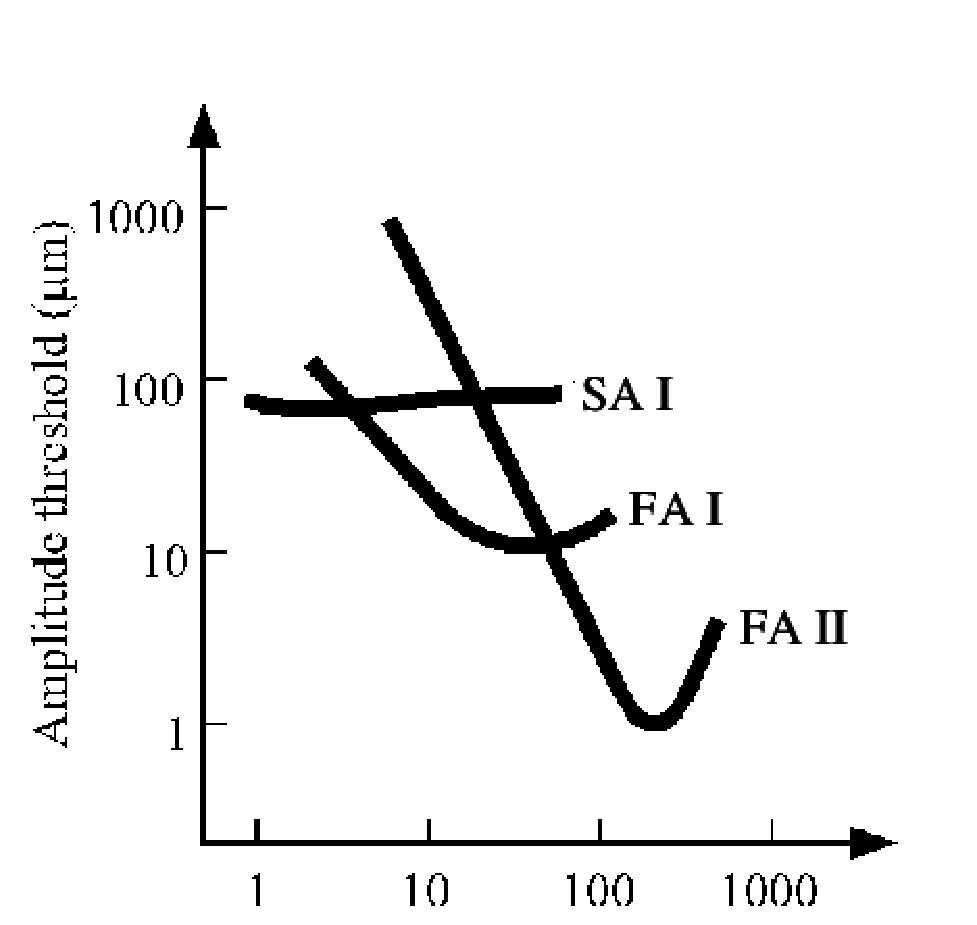
\includegraphics[width=8cm]{eps/threshold.eps}
    \caption{受容器の振動検出(\cite{maeno}より)}
    \label{fig:rece}
   \end{center}
   \end{figure}
   
\section{触覚情報の取扱に関する研究}
触覚ディスプレイを用いた情報提示の前段階として, テクスチャの触覚データを加速度情報として取得する研究が広く行われている.  Abdulali らは収集した加速度触覚情報をニューラルネットワークの1種である Radial Basis Function Network を用い分類を行った\cite{abdulalis}.   Strese らはユークリッド距離, マハラノビス距離, GMM の3種の機械学習アルゴリズムをそれぞれを使用し分類を行い, 精度比較を行っている\cite{strese2016multimodal}. また, Jamali らは単純ベイズ分類器を用いて分類を行った \cite{jamali2010material}. 
また, 機械学習で分類を行うにあたって, 入力に次元削減を施している研究も見受けられる. 
 Mengqi らはオートエンコーダと畳み込みニューラルネットワークを組み合わせた ACNN というネットワークを用い分類を行っている\cite{mengqi}. この際用いられている手法が J. Kuchenbecker らによって提案された DFT321 \cite{dft321} と呼ばれる次元削減アルゴリズムである. この手法は同様に畳み込みニューラルネットワークで触覚情報の分類を行った Zheng ら \cite{zheng2016deep} やTawfique ら \cite{Tawfique} も入力の前処理として使用している. しかし, 同じ3軸加速度データを扱う研究でも人の行動分析の場合, 3軸加速度をそのまま入力とする研究も多く見られる \cite{active_recog}. 
 
 これらの先行研究に対し, 本研究ではテクスチャの分類問題に対して, 次元削減の妥当性の検証として基本的かつシンプルな畳み込みニューラルネットワークを構築し, 次元削減を行った場合の3軸加速度触覚情報と次元削減を行わない場合の3軸加速度触覚情報で分類精度の観点から性能にどの程度差が生じるか比較を行う. また, 畳み込みニューラルネットワークで一般に用いられる特徴量ごとの正規化を3軸加速度触覚情報にも適用し, 正規化を行わない場合の分類精度との比較を行う.

% Local Variables:
% TeX-master: "main"
% mode: yatex
% End:


%#!platex --src-specials main.tex

\chapter{触覚情報の次元削減手法と\\機械学習}
\label{chap:method}
本章では,\ref{sec:prepro}にて加速度触覚データの分類に用いた3軸加速度データの前処理について記述する . \ref{sec:cnn}にて触覚情報分類に用いる畳み込みニューラルネットワークの概説を行う. 
\section{触覚情報の次元削減手法}
\label{sec:prepro}
次元削減を行った3軸加速度触覚データと次元削減を行わず正規化を施した3軸加速度触覚データ, 次元削減を行わず正規化も行わない3軸加速度触覚データのうち, どの取り扱い手法が分類に適しているかを調査するため, それぞれのアルゴリズムで前処理した加速度触覚データを作成した. 
対象としたデータは J. Kuchenbecker によって提案された DFT321 \cite{dft321} の論文中に比較検討対象として上がっていた5つのアルゴリズムによって次元削減された1軸の触覚データと, 各軸ごとに大きさを0から1の間で正規化した3軸加速度触覚データ, 何も施さない3軸加速度触覚データである. 前処理工程の末尾に付く321という文字は 3-dimensions to 1-dimension の略である. 
\subsection{比較対象アルゴリズム}
\subsubsection{Single - Axis : SA321}
SA321について説明する. これはセンサによって得られた3軸データのうち, 1軸のデータのみを抽出して扱う手法である. 
これについて, センサのx,y,z軸に対してそれぞれの信号を$SA321-x$, $SA321-y$, $SA321-z$とし3つの1軸データとして取り扱う.  
テスクチャに対しての鉛直方向や移動軸に対して分類を決定づける特徴がでると想定できるが, 単純にx,y,z軸に沿って現れるという保証はないため大幅な信号損失の可能性が問題となる.  

\subsubsection{Sum of Components : SoC321}
SoC321 について説明する. これは3軸加速度データの$x$,$y$,$z$成分を単純加算し, 1つの信号として扱う手法である. 3軸信号を$a(t)$とすると, 
\begin{equation}
SoC321(a)=a_{x}+a_{y}+a_{z} 
\end{equation}
計測するテクスチャに特徴的な振動があれば指自体が何かしらの挙動を起こし, 取り付けられた加速度センサも3軸同時に特徴的な振動を計測できるため, 3軸間の時間的相関は考えられる. 
ただし3軸加速度データを取り扱う上で, 正の向きや負の向きの加速度は軸が違えば単純に比較できないことは明白であるが, SoC321 において加速度を単純加算しているため, 正負の振動の情報に対して有意な値を保持することができない可能性がある. 

\subsubsection{Vector Magnitude : Mag321}
Mag321 について説明する.これは3軸加速度データの$x$,$y$,$z$成分に対してそれぞれ2乗し平方根をとったものを, 1つの信号として扱う手法である. 
\begin{equation}
Mag321(a)=\sqrt{{a_{x}}^2+{a_{y}}^2+{a_{z}}^2} 
\end{equation}
これは前述の正や負の加速度の向きを考慮せずベクトルの大きさのみに情報を絞って扱っているため, それぞれの軸の絶対的な振動のスケール情報は残る. しかしこれも正負の振動情報に対して有意な値が保持できない可能性がある.

\subsubsection{主成分分析 (Principal Component Analysis, PCA)}
主成分分析 (PCA) について概説する. これは代表的な次元圧縮方法であり, 以下の流れで計算を行う. 
\begin{enumerate}
  \item 全データの平均を求める
  \item 平均に対してデータの分散が最大のベクトルを探索
  \item 新しい表現軸として, 先程求めたベクトルを基底とするベクトルを設定
  \item 上記でとった軸の直交ベクトルに対して分散が最大となるベクトルを探す
  \item データの軸の分だけ繰り返す
\end{enumerate}
これを実際の計算に落とし込むと以下のようになる. 
まず, データ${x_{i} = (x_{i1}, .. , x_{id})^{\mathrm{T}}(i = 1, .. ,N)}$
に対して, データ行列${X = (x_{1}, .. ,x_{N})^{\mathrm{T}}}$の偏差${\bar{X}=(x_{1} - \bar{x} .. ,x_{N} - \bar{x})^{\mathrm{T}}}$を定義する. ここで求める単位ベクトル$a$を${a = (a_{1}, .. ,a_{d})^{\mathrm{T}}}$とすると, 
ここから分散$Var({\bar{Xa}})$は以下のように導ける. 
\begin{equation}
Var({\bar{Xa}}) = \frac{1}{N}(\bar{Xa})^{\mathrm{T}}(\bar{Xa}) = \frac{1}{N}{a}^T\bar{X}^{\mathrm{T}}\bar{Xa} = a^TVar({{\bar{X}}})a
\end{equation}
この分散を最大化する$a$を求めるには, $a$のノルムを1とする制約をつけ, ラグランジュ未定乗数法を適用する. 式を
\begin{equation}
{G(a) = a^{\mathrm{T}}Var({{\bar{X}}})a - \lambda(a^{\mathrm{T}} a - 1)} 
\end{equation}
と置き, $a$で偏微分すると次の式が得られる. 
\begin{equation}
{\frac{\partial G(a)}{\partial a} = 2 Var({{\bar{X}}})a - 2\lambda a = 0}
{Var (\bar{X})a = \lambda a}
\end{equation}
この等式から最大固有値$\lambda$に属する固有ベクトルを求め$a$とすると, 主成分を求める事ができる. 

\subsubsection{Discrete Fourier Transform : DFT321}
DFT321\cite{dft321}について説明する. DFT321 は J.Kuchenbecker によって提案された離散フーリエ変換 ( Discrete Fourier Transform : DFT )をもとにした次元削減アルゴリズムである. 
高周波振動に対するヒトの触覚検知は信号のスペクトル成分に依存する\cite{dft321}ため, 次元削減を行う際に理想となるのは元の3軸信号のエネルギースペクトル密度 (Energy Spectrum Density : ESD) を保存されることとしている. しかし, 無加工の3軸加速度データに対して高速フーリエ変換 (Fast Fourier Transform : FFT) 後生成されたスペクトルにはノイズが多いため, 各周波数におけるエネルギースペクトル密度からスペクトルの類似性を直接判断することは難しい. そこで DFT321 では得られたスペクトルに対して, パチニ小体がより振動刺激を感じ取れるとされる\, 20$-$1000\, $\mathrm{Hz}$の間のみを抽出し平滑化をかける. 3軸信号${a(t)}$のスペクトル信号を${{A}(f)}$, 平滑化をしたものを${\tilde{A}(f)}$, 次元削減後の1軸信号を${\tilde{A}_{s}(f)}$とし, 次元削減前の3軸信号と次元削減後の1軸信号とのスペクトルの類似度を表すためスペクトル一致距離${M_{sm}}$を以下に定義している. 

\begin{equation}
{M_{s m}=1-\frac{1}{n_{f}} \sum_{f=20 H_{z}}^{1000 H z}\left(\frac{\left|\tilde{A}_{x}(f)\right|^{2}+\left|\tilde{A}_{y}(f)\right|^{2}+\left|\tilde{A}_{z}(f)\right|^{2}-\left|\tilde{A}_{s}(f)\right|^{2}}{\left|\hat{A}_{x}(f)\right|^{2}+\left|\tilde{A}_{y}(f)\right|^{2}+\left|\tilde{A}_{z}(f)\right|^{2}}\right)}
\end{equation}


またESDが同等でも, 時間軸上で次元削減前に比べて差異があると理想的な次元削減が行われてるとは言い難い. この問題を解決するため, DFT321 では時間的なズレに対する簡単な尺度として, 次元削減前の3軸信号と次元削減後の1軸信号との間のゼロ遅延の相互相関を用いた評価を行う. 相関関数には正負の値が存在するが, 負の場合2つの信号の間に逆相関の関係があることを示す. これは振動の向きでいうと逆であることを示すが, 人間の手は振動の方向に敏感ではないとされていることから相関の正負は無視できると考える. したがって実際には前述のゼロ遅延の相互相関の絶対値を用いる以下の式により時間的一致距離${M_{tm}}$を定義する. ここで$\star$はゼロ遅延での相互相関を示す. 

\begin{equation}
{M_{t m}=\frac{1}{3}\left(\frac{\left|a_{x} \star a_{s}\right|}{\sqrt{a_{x} \star a_{x}} \sqrt{a_{s} \star a_{s}}}+\frac{\left|a_{y} \star a_{s}\right|}{\sqrt{a_{y} \star a_{y}} \sqrt{a_{s} \star a_{s}}}+\frac{\left|a_{z} \star a_{s}\right|}{\sqrt{a_{z} \star a_{z}} \sqrt{a_{s} \star a_{s}}}\right)}
\end{equation}


上述した他のアルゴリズムでは上記2つの$M_{sm}$, $M_{t m}$に対して考慮がなされた設計がされているとは言い難いため, DFT321 では DFT を用い信号スペクトルに対して操作を行うことで上記2つの$M_{sm}$, $M_{t m}$を考慮し設計されている. 
まずは次元削減後のベクトルの大きさ$\left|\tilde{A}_{s}(f)\right|$についてのみ考える. 
上述の$M_{sm}$の式から, 分子部分の
\begin{equation}
{\left|\tilde{A}_{x}(f)\right|^{2}+\left|\tilde{A}_{y}(f)\right|^{2}+\left|\tilde{A}_{z}(f)\right|^{2}-\left|\tilde{A}_{s}(f)\right|^{2}}
\end{equation}

が0に近いほど$M_{sm}$は大きい値を取る. そこで次元削減後のベクトル${\tilde{A}_{s}(f)}$の大きさ$\left|\tilde{A}_{s}(f)\right|$は以下で計算する. 

\begin{equation}
{\left|\tilde{A}_{s}(f)\right|=\sqrt{\left|\tilde{A}_{x}(f)\right|^{2}+\left|\tilde{A}_{y}(f)\right|^{2}+\left|\tilde{A}_{z}(f)\right|^{2}}}
\end{equation}


次に次元削減後のベクトルの位相$\theta_{f}$について考える. 
周波数領域上ではゼロ遅延相互相関を以下で表すことができる. 
\begin{equation}
\sum_{i=1}^{3} a_{i} \star a_{s}
\end{equation}


上記より, ${\tilde{A}_{s}(f)}$の位相は以下の場合に$M_{t m}$において最大値を得る位相$\theta_{f}^{max}$を取る. 
\begin{equation}
{\theta_{f}^{\max }=\angle \sum_{i=1}^{3} \tilde{A}_{i}}
\end{equation}

$\left|\tilde{A}_{s}(f)\right|$と$\theta_{f}^{max}$により得られる合成信号${\left|\tilde{A}_{s}(f)\right|e^{j \theta_{f}^{\max }}}$に逆離散フーリエ変換(Inverse DFT : IDFT) を施して実部の値をとったものをDFT321で得られる次元削減後の信号${\tilde{A}_{s}(f)}$として得ることができる. 

\begin{equation}
{{\tilde{A}_{s}(f) = Real[{F^{-1}({\left|\tilde{A}_{s}(f)\right|e^{j\theta_{f}^{\max }}})}]}}
\end{equation}

\subsubsection{正規化}
正規化について説明する.これは3軸加速度データの$x$,$y$,$z$成分を軸ごとに0から1の間にスケーリングし直す処理である. 
機械学習においてデータセットの特徴量間でスケールが異なることがある場合, パラメータ間の更新幅に偏りが生じることで学習結果や計算時間に悪影響を及ぼすことがある. これを防ぐため, データ軸ごとに正規化を行い, 更新幅を揃え分類精度の向上を期待する.$x$軸の場合, $i$番目の値$x_{i}$は以下の式で正規化される. 

\begin{equation}
    {x_ {norm,i}=\frac{x_{i}-x_{\min }}{x_{\max }-x_{\min }}}
\end{equation}

\section{畳み込みニューラルネットワーク}
\label{sec:cnn}
本実験において, 加速度触覚情報の分類のため畳み込みニューラルネットワーク (Convolutional Neural Network: CNN) を用いる.  
CNN は, 近年特に機械学習分野への関心が高まる一因となった画像認識タスクにおいて突出した成果を収めているニューラルネットワークの一種である.  
生物の脳の視覚神経系の構造から単細胞層と複雑細胞層を組み合わせた2層の神経回路を基本モジュールとしてモデル化した, Fukushima らが発案した Neocognitron \cite{fukushima1983neocognitron} を発展させたものとして知られている. Neocognitron において重要な役割を果たすアイデアに, 局所特徴量の考慮が挙げられる. これは入力側により近い浅い層において, 比較的狭い範囲の近い点の集合から得た特徴を統合抽出し次の層に伝搬を行うことで実現している. その後 Y. LeCun らによって Neocognitron のモデルを誤差逆伝搬法による勾配計算によって教師あり学習に改良した CNN が提唱された \cite{lecun}. 
このCNNは画像認識以外にも様々なタスクに有効であることが確認されており, 自然言語処理\cite{NLP}から金融\cite{finance}や人間の行動認識\cite{active_recog}\cite{chen2015deep}等時系列データの分類にも適用事例が多数報告されている. 

CNN の基本構成を以下の図\ref{fig:cnn_std}に示す. 
\begin{figure}[H]
    \begin{center}
    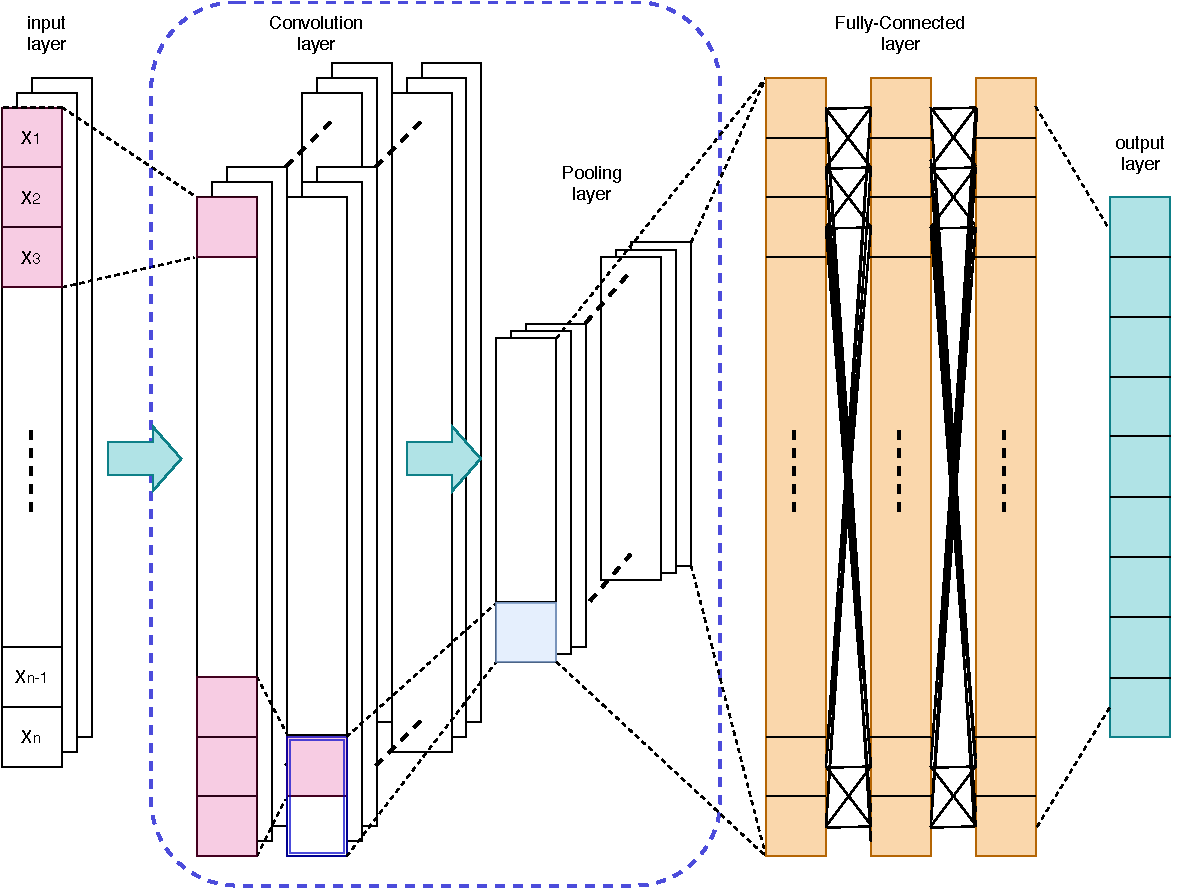
\includegraphics[width=12cm]{eps/cnn_architecture.pdf}
    \caption{CNNの基本構成}
    \label{fig:cnn_std}
   \end{center}
   \end{figure}
前述の Neocognitron 同様, 入力側に近い浅い層で特徴抽出を行うため, 畳み込みとプーリング処理を複数回行い特徴を計算する. 出力側に近い深い層で識別を行う. ネットワークの最終層では分類を行う各クラスごとの制度を算出するための出力層が追加される. 

\subsection{1次元の畳み込み処理}
畳み込み層がない従来のニューラルネットワークの場合, 入力の形式に問わず並列に扱ってしまう問題点がある. 例えば入力が画像である場合, あるピクセルと近傍のピクセル値は似た値になることが多く逆に離れた点同士には近傍のピクセルほどパターンや傾向を見いだせないことが多い. 時系列データの場合でも計測している事象が時間軸上で連続しており, 近傍点は似た値に, 離れた点はそうではない事が考えられる. このようにある一点において, 距離的に近いところとでなすはずの特徴を従来のニューラルネットワークでは捉えきれない可能性がある. 
前述の通り, 局所特徴量の抽出に優れた CNN の方が時系列データにおけるパターンに関する重要な特徴を捉えきれる可能性が高く有用だと考えた. 

畳み込み層で行う処理について説明する. 
畳み込み演算は入力データに対してフィルタ(カーネル)を適用する. 
本研究では入力データは1軸または3軸の時系列データであるため,  CNN の中でも1次元の畳み込み層を持つ 1D CNN を用いている. 
長さ$W$の1次元データに対する畳み込みを考える. 1つのデータ点をインデックス$i$を用いて$x_{i}$と表す. また同様に長さ$H$のフィルタ(カーネル)に対しても1つのフィルタ点をインデックス$p$を用いて$h_{p}$と表す. これらを積和演算することで畳み込み処理後のデータが得られる. 
\begin{equation}
{u_{i}=\sum_{p=0}^{H-1} x_{i+p} h_{p}}
\end{equation}

次にチャネルについて考える. 
チャネル番号$ k(= 0, 1, 2, 3, ..., K − 1)$とおく. 入力データが3軸である場合, チャネルはx, y, z軸方向データの K = 3と考えることができる. これを用い前述の式を拡張する. 
\begin{equation}
{u_{i}=\sum_{k=0}^{K-1}\sum_{p=0}^{H-1} x_{i+p,k} h_{pk}}
\end{equation}

次に畳み込み演算を行う層について考える. 
第 $l$ 層の畳込み層について, 前層$l − 1$ 層の出力$z^{(l-1)}_{ik}$に M 種類のフィルタ $h_{pkm}(m =
0, 1, 2, 3, ..., M − 1)$ を適用し, バイアス$ b_{m}$ を考慮するとフィルタからからの出力$u_{im}$は以下の式で定義される. 
\begin{equation}
{u_{im}=\sum_{k=0}^{K-1}\sum_{p=0}^{H-1} z^{(l-1)}_{i+p,k,m} h_{pkm}+b_{m}}
\end{equation}

活性化関数$f$を定義し, フィルタからの出力$u_{im}$をかけ合わせた畳み込み層の出力$z^{(l)}_{im}$を得る. 
\begin{equation}
{z^{(l)}_{im}=f(u_{im})}
\end{equation}

1次元畳み込み演算を以下の図\ref{fig:1dconv}に示す. 
\begin{figure}[H]
    \begin{center}
    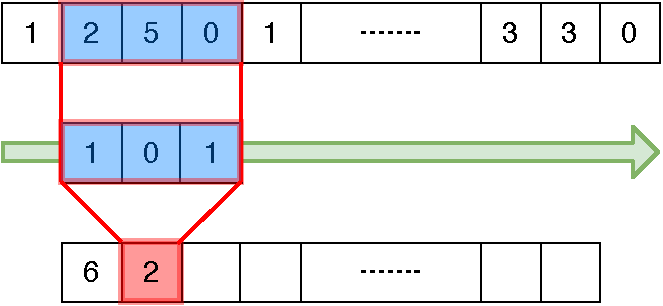
\includegraphics[width=12cm]{eps/1dconv.pdf}
    \caption{1次元畳み込み演算}
    \label{fig:1dconv}
   \end{center}
   \end{figure}

\subsection{1次元プーリング}
CNN において, プーリング層は畳み込み層と併せて使用される. 
主に畳み込み層で得た局所特徴に圧縮を行うような形で使用されることが多く, そのため畳み込み層の後層に配置される. 情報の圧縮を行う事により, フィルタ形状の位置ずれをある程度許容し, かつ計算量を抑えるという効果が期待できる. 
構造はシンプルであり, ある局所領域から代表値を抽出することで実現される. 
代表的な手法に局所領域中から最大値を取り出す最大プーリングが挙げられる. 

1次元最大プーリングを以下の図\ref{fig:1dpool}に示す. 

\begin{figure}[H]
    \begin{center}
    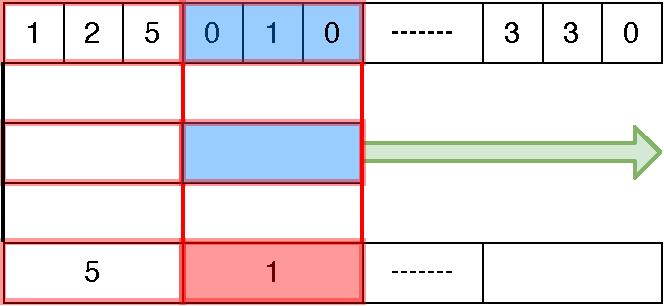
\includegraphics[width=12cm]{eps/1dpool.pdf}
    \caption{1次元最大プーリング処理}
    \label{fig:1dpool}
   \end{center}
   \end{figure}

% Local Variables:
% TeX-master: "main"
% mode: yatex
% End:


%#!platex --src-specials main.tex
\chapter{評価実験}
\label{chap:exp}
本章では実施した評価実験について述べる. 
\section{実装}
加速度触覚情報を分類するにあたって実装した CNN モデルについて説明する. 
この 1D CNN の構造は同じ時系列センサデータの分類を比較的小規模なネットワークで実現した Mumtaz らの研究\cite{mumtaz}や Priyadarshiniら\cite{priyadarshini} のモデルを参考に調整を行った. 

\subsection{入力データ}
入力データは Agatsuma ら\cite{agatsuma}が作成した3軸加速度データを使用した. 
9種のテクスチャに対しそれぞれ約5秒間以上指の腹でなぞった際の指先の振動を3軸加速度センサで計測したデータであり, サンプリング周波数は$1 \, \mathrm{kHz}$ である. また1テクスチャあたり80セットのデータを有す. 
分類を行うにあたり, データのうち最初の500点までと4,596点以降のデータをトリムし全4,096点のデータに整形したものを前処理にかけ,  CNN の入力に用いる. 

\begin{figure}[H]
    \begin{center}
    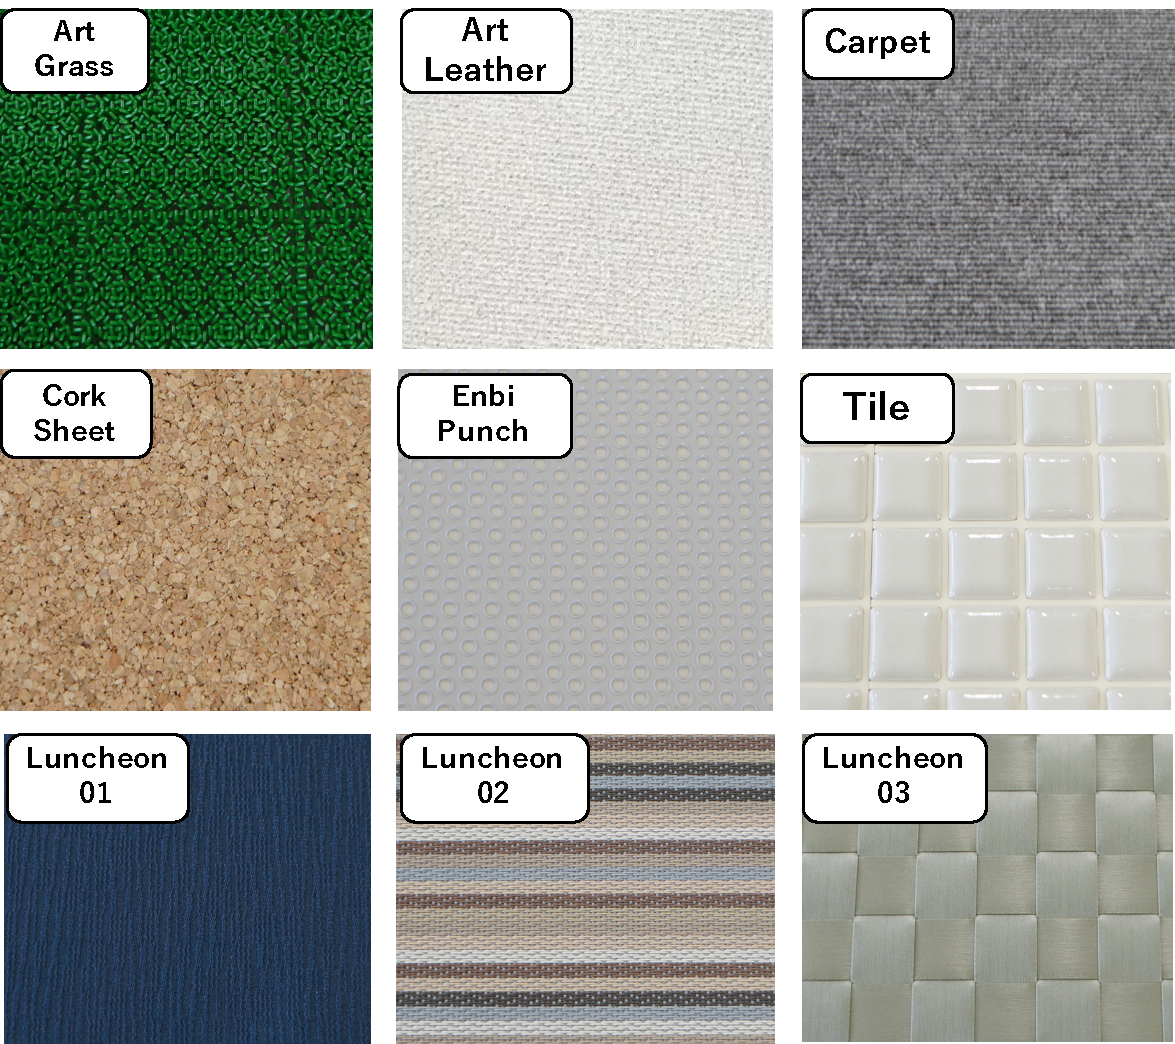
\includegraphics[width=12cm]{eps/textures.pdf}
    \caption{使用した9種のテクスチャ外観}
    \label{fig:texture}
   \end{center}
   \end{figure}

\begin{figure}[H]
    \begin{center}
    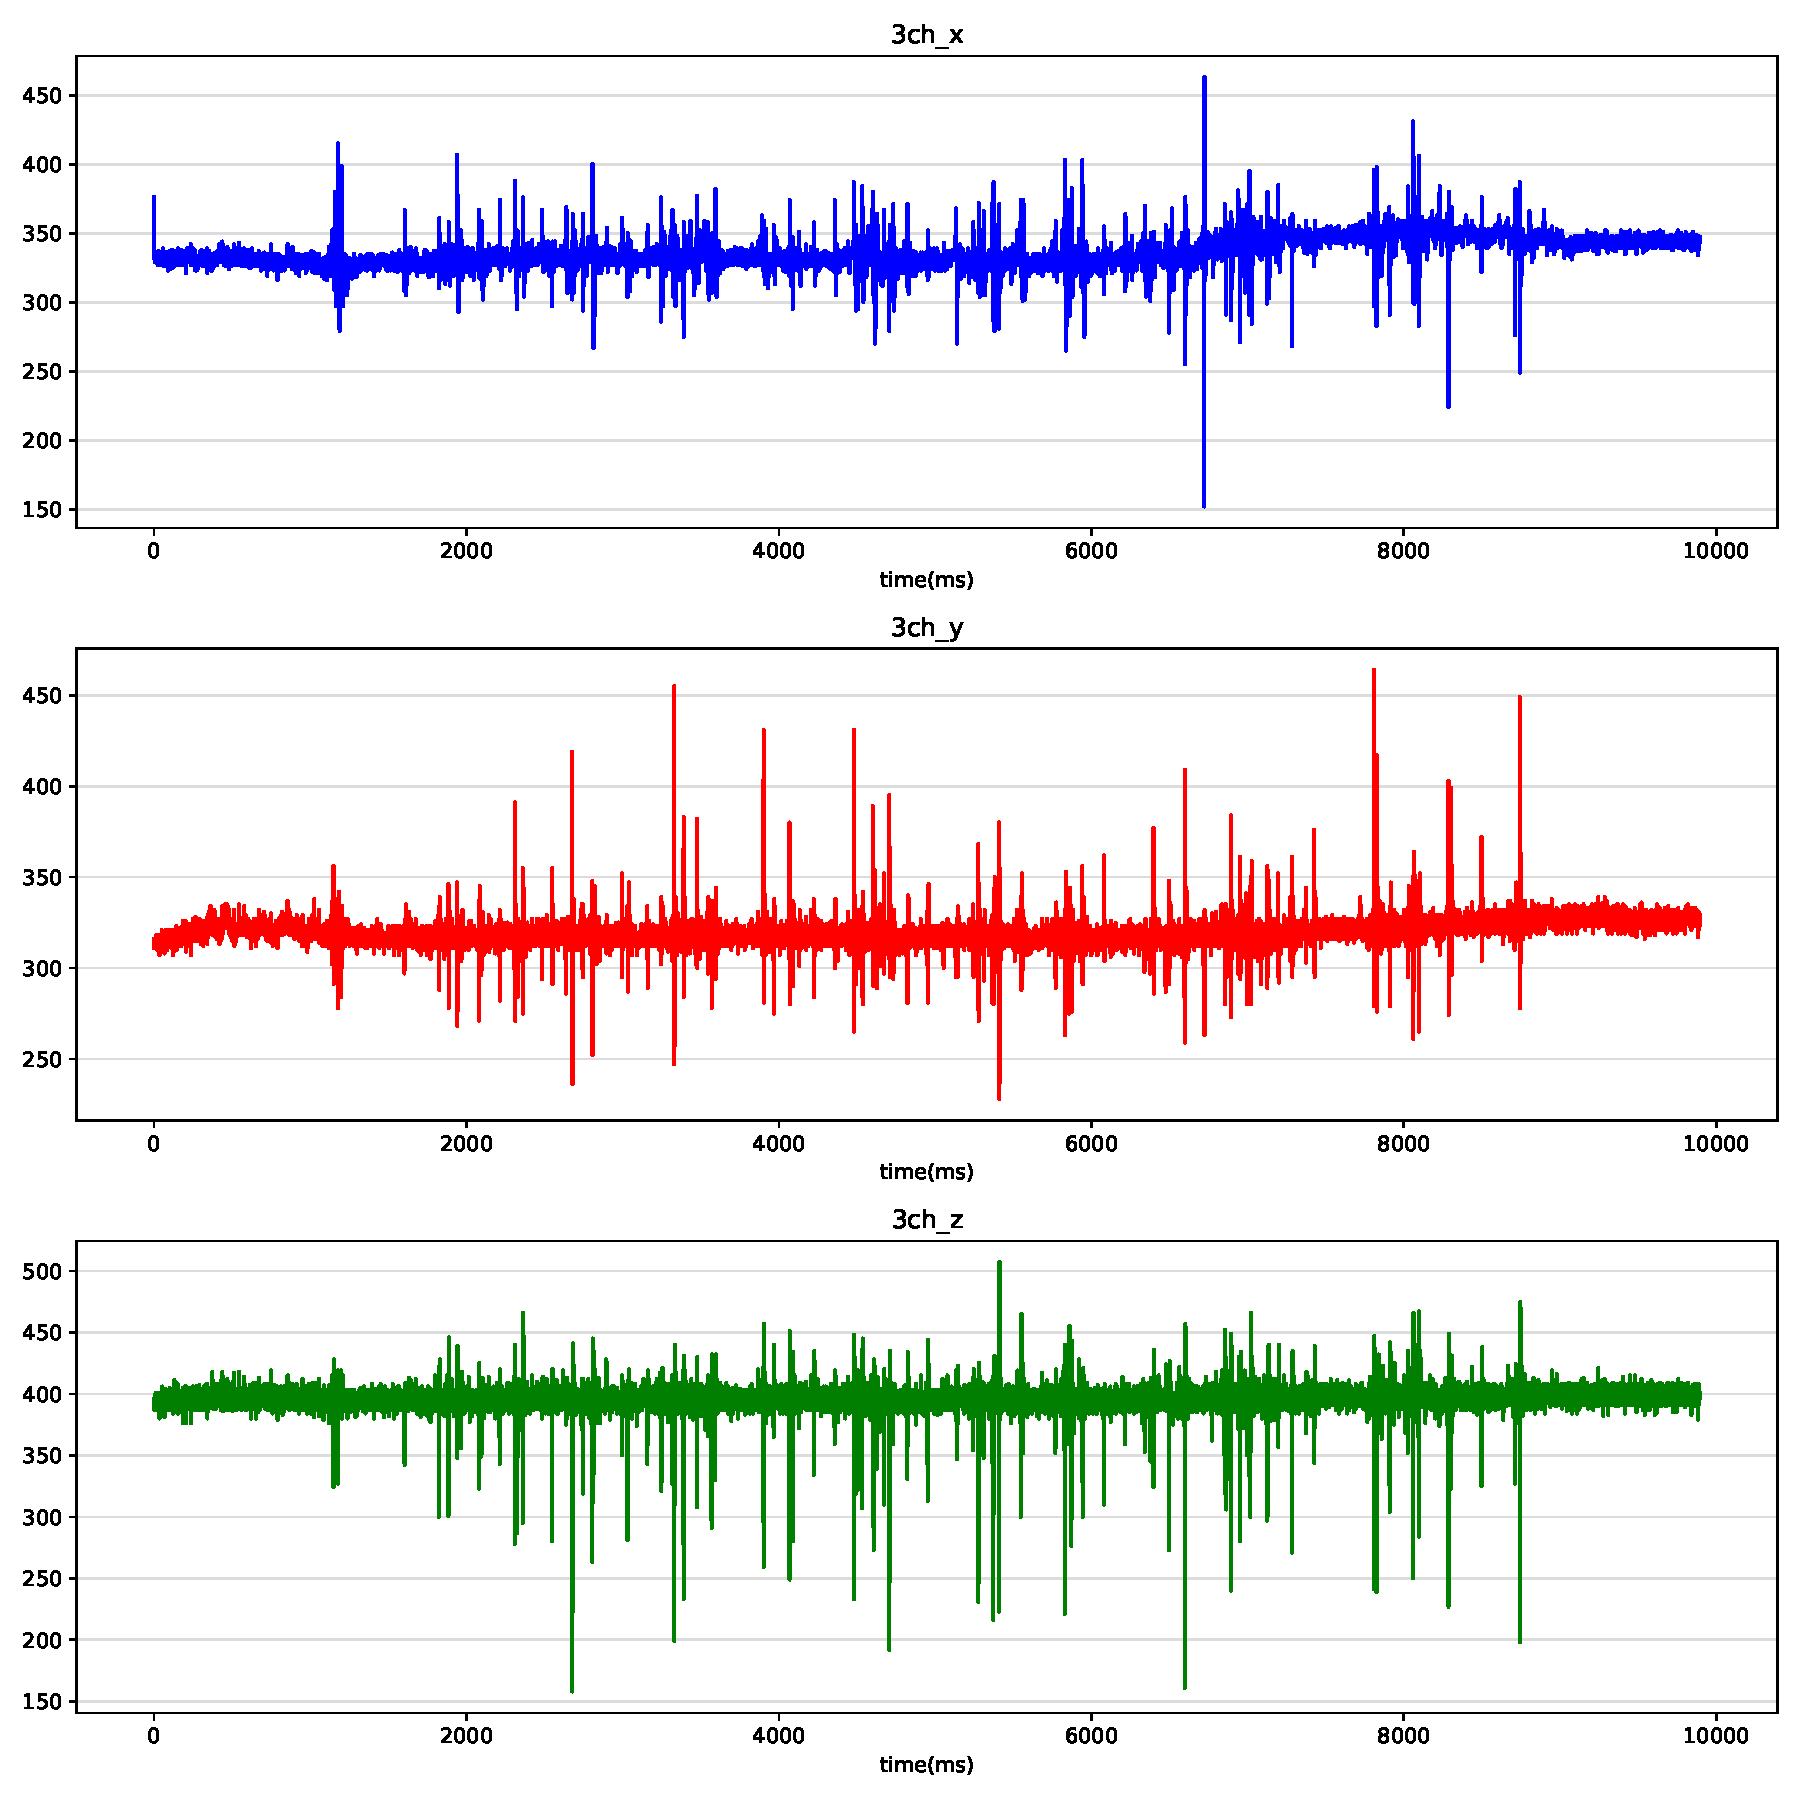
\includegraphics[width=12cm]{eps/3ch.pdf}
    \caption{Art Grass をなぞった際の3軸加速度データ(x,y,z)の例}
    \label{fig:3ch}
   \end{center}
   \end{figure}

\subsection{前処理}
一部の整形したデータは, 比較評価のため上述の各アルゴリズムで次元削減または正規化を行う. 
それぞれの前処理を施した Art Grass をなぞった際の3軸加速度データを各アルゴリズムで次元削減した信号の例を SoC321, Mag321, PCA, DFT321 の順で以下の図\ref{fig:prepros}に示す. 

\begin{figure}[H]
    \begin{center}
    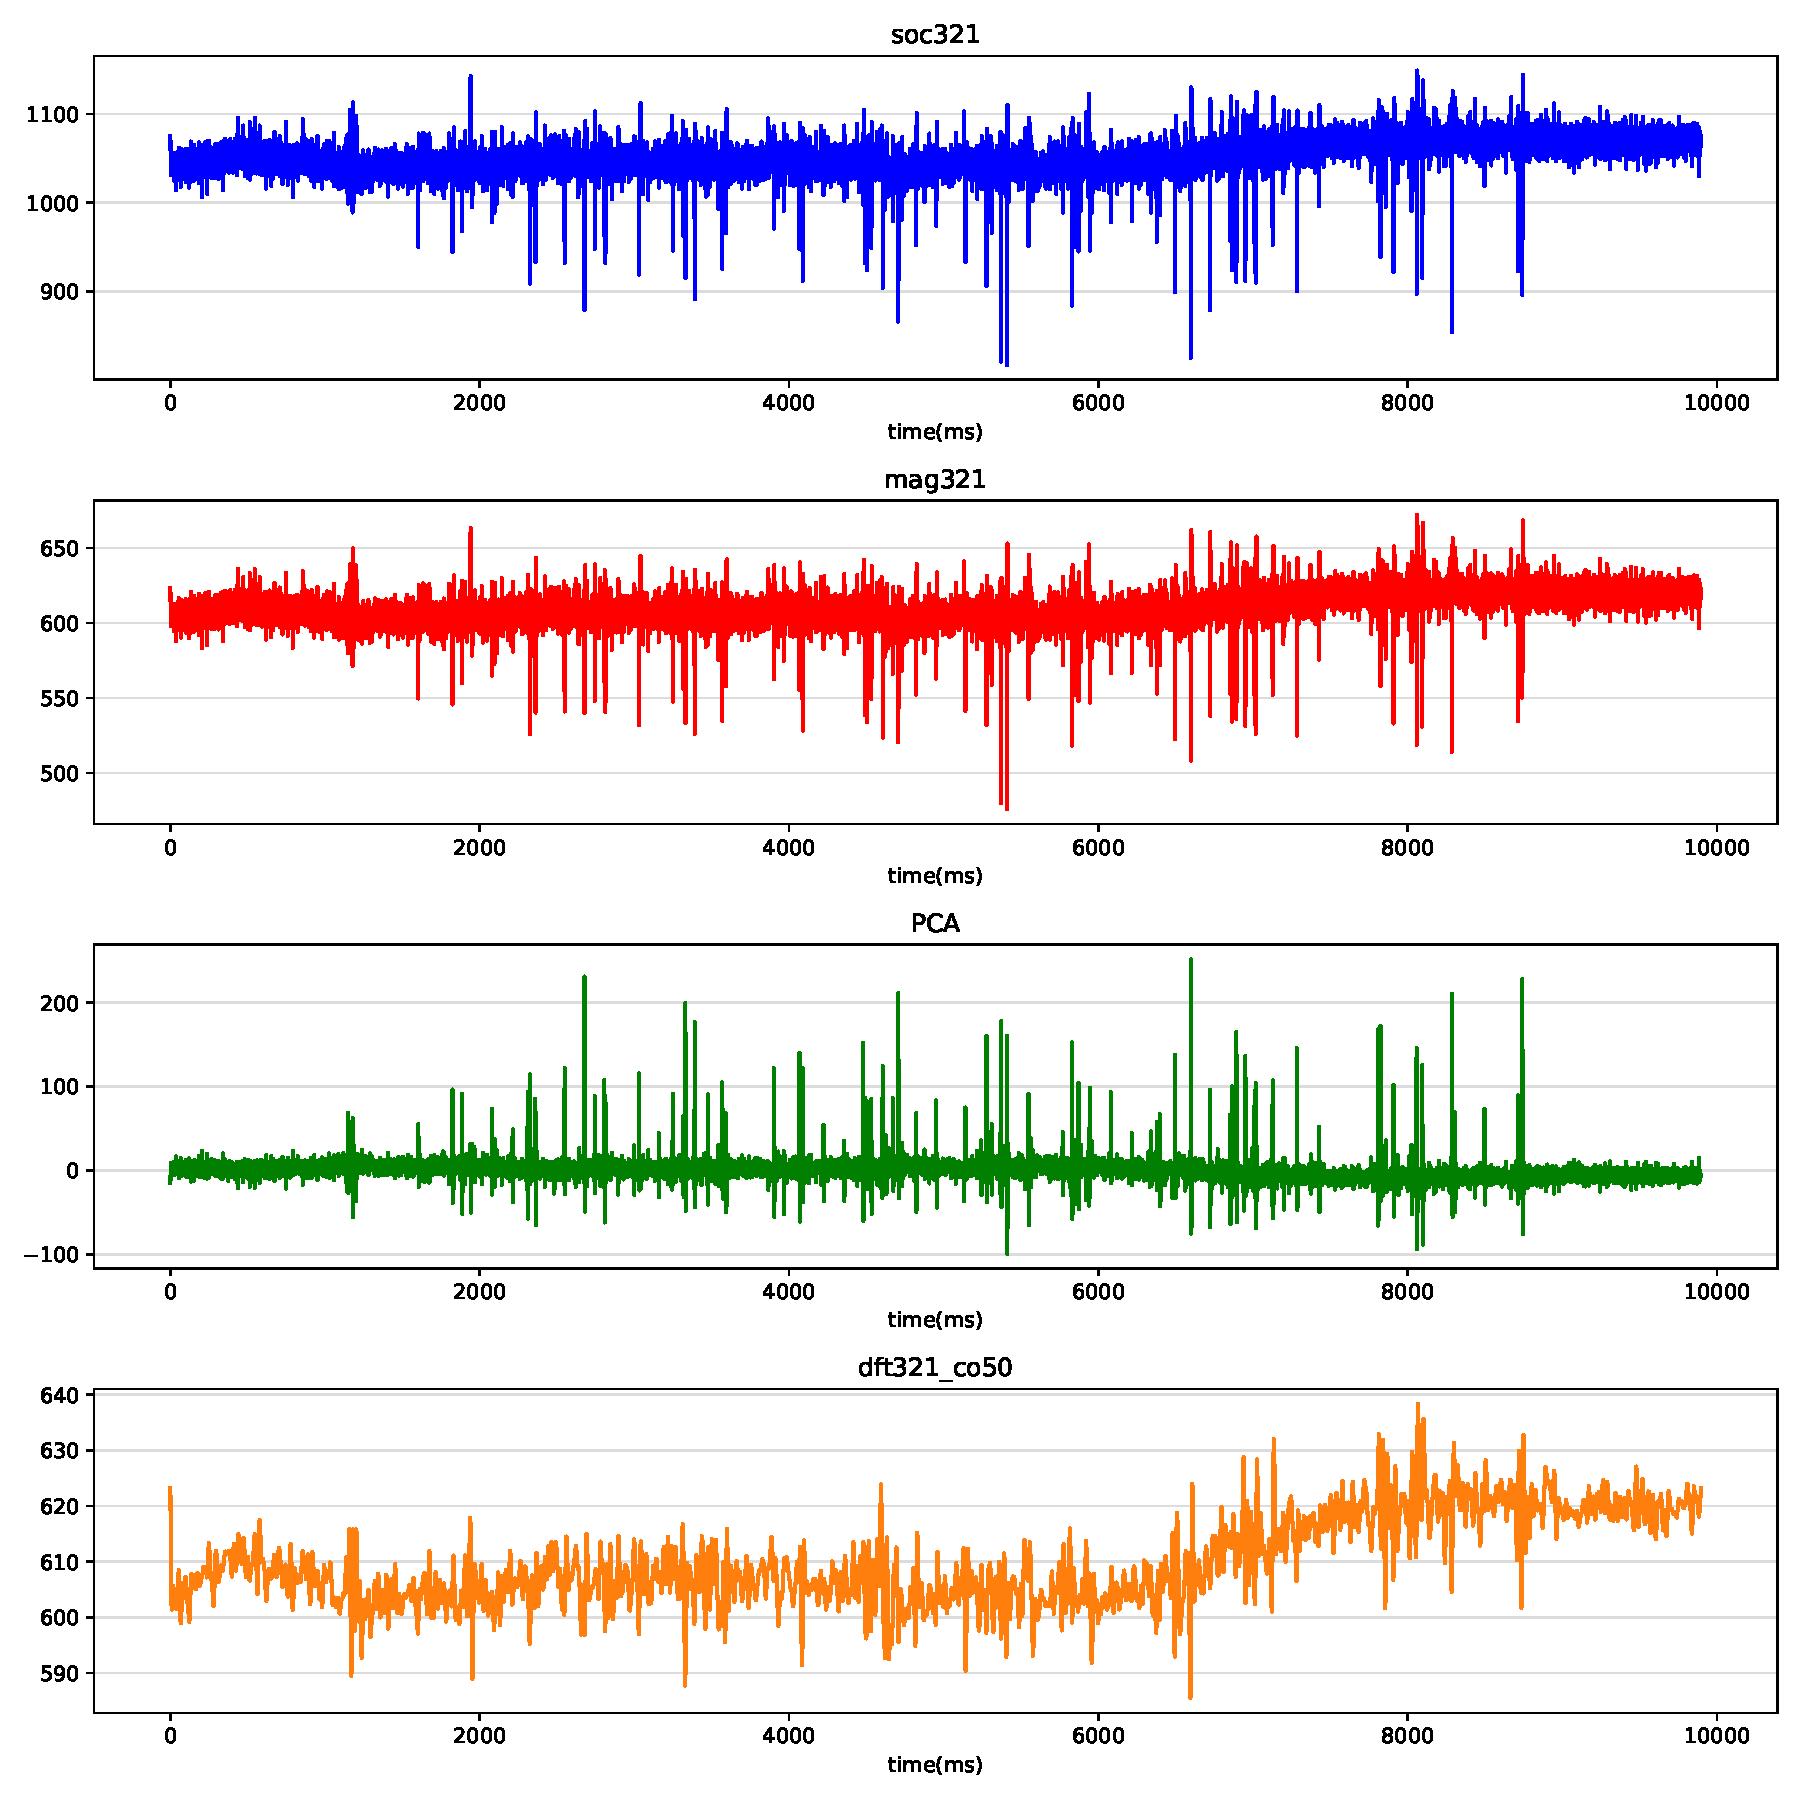
\includegraphics[width=12cm]{eps/1ch_4.pdf}
    \caption{Art Grass をなぞった際の3軸加速度データに各次元削減アルゴリズムを適用した場合の出力信号例}
    \label{fig:prepros}
   \end{center}
   \end{figure}
   
また, 同様に正規化を行った3軸加速度データの信号例を以下の図\ref{fig:normalize}に示す. 

\begin{figure}[H]
    \begin{center}
    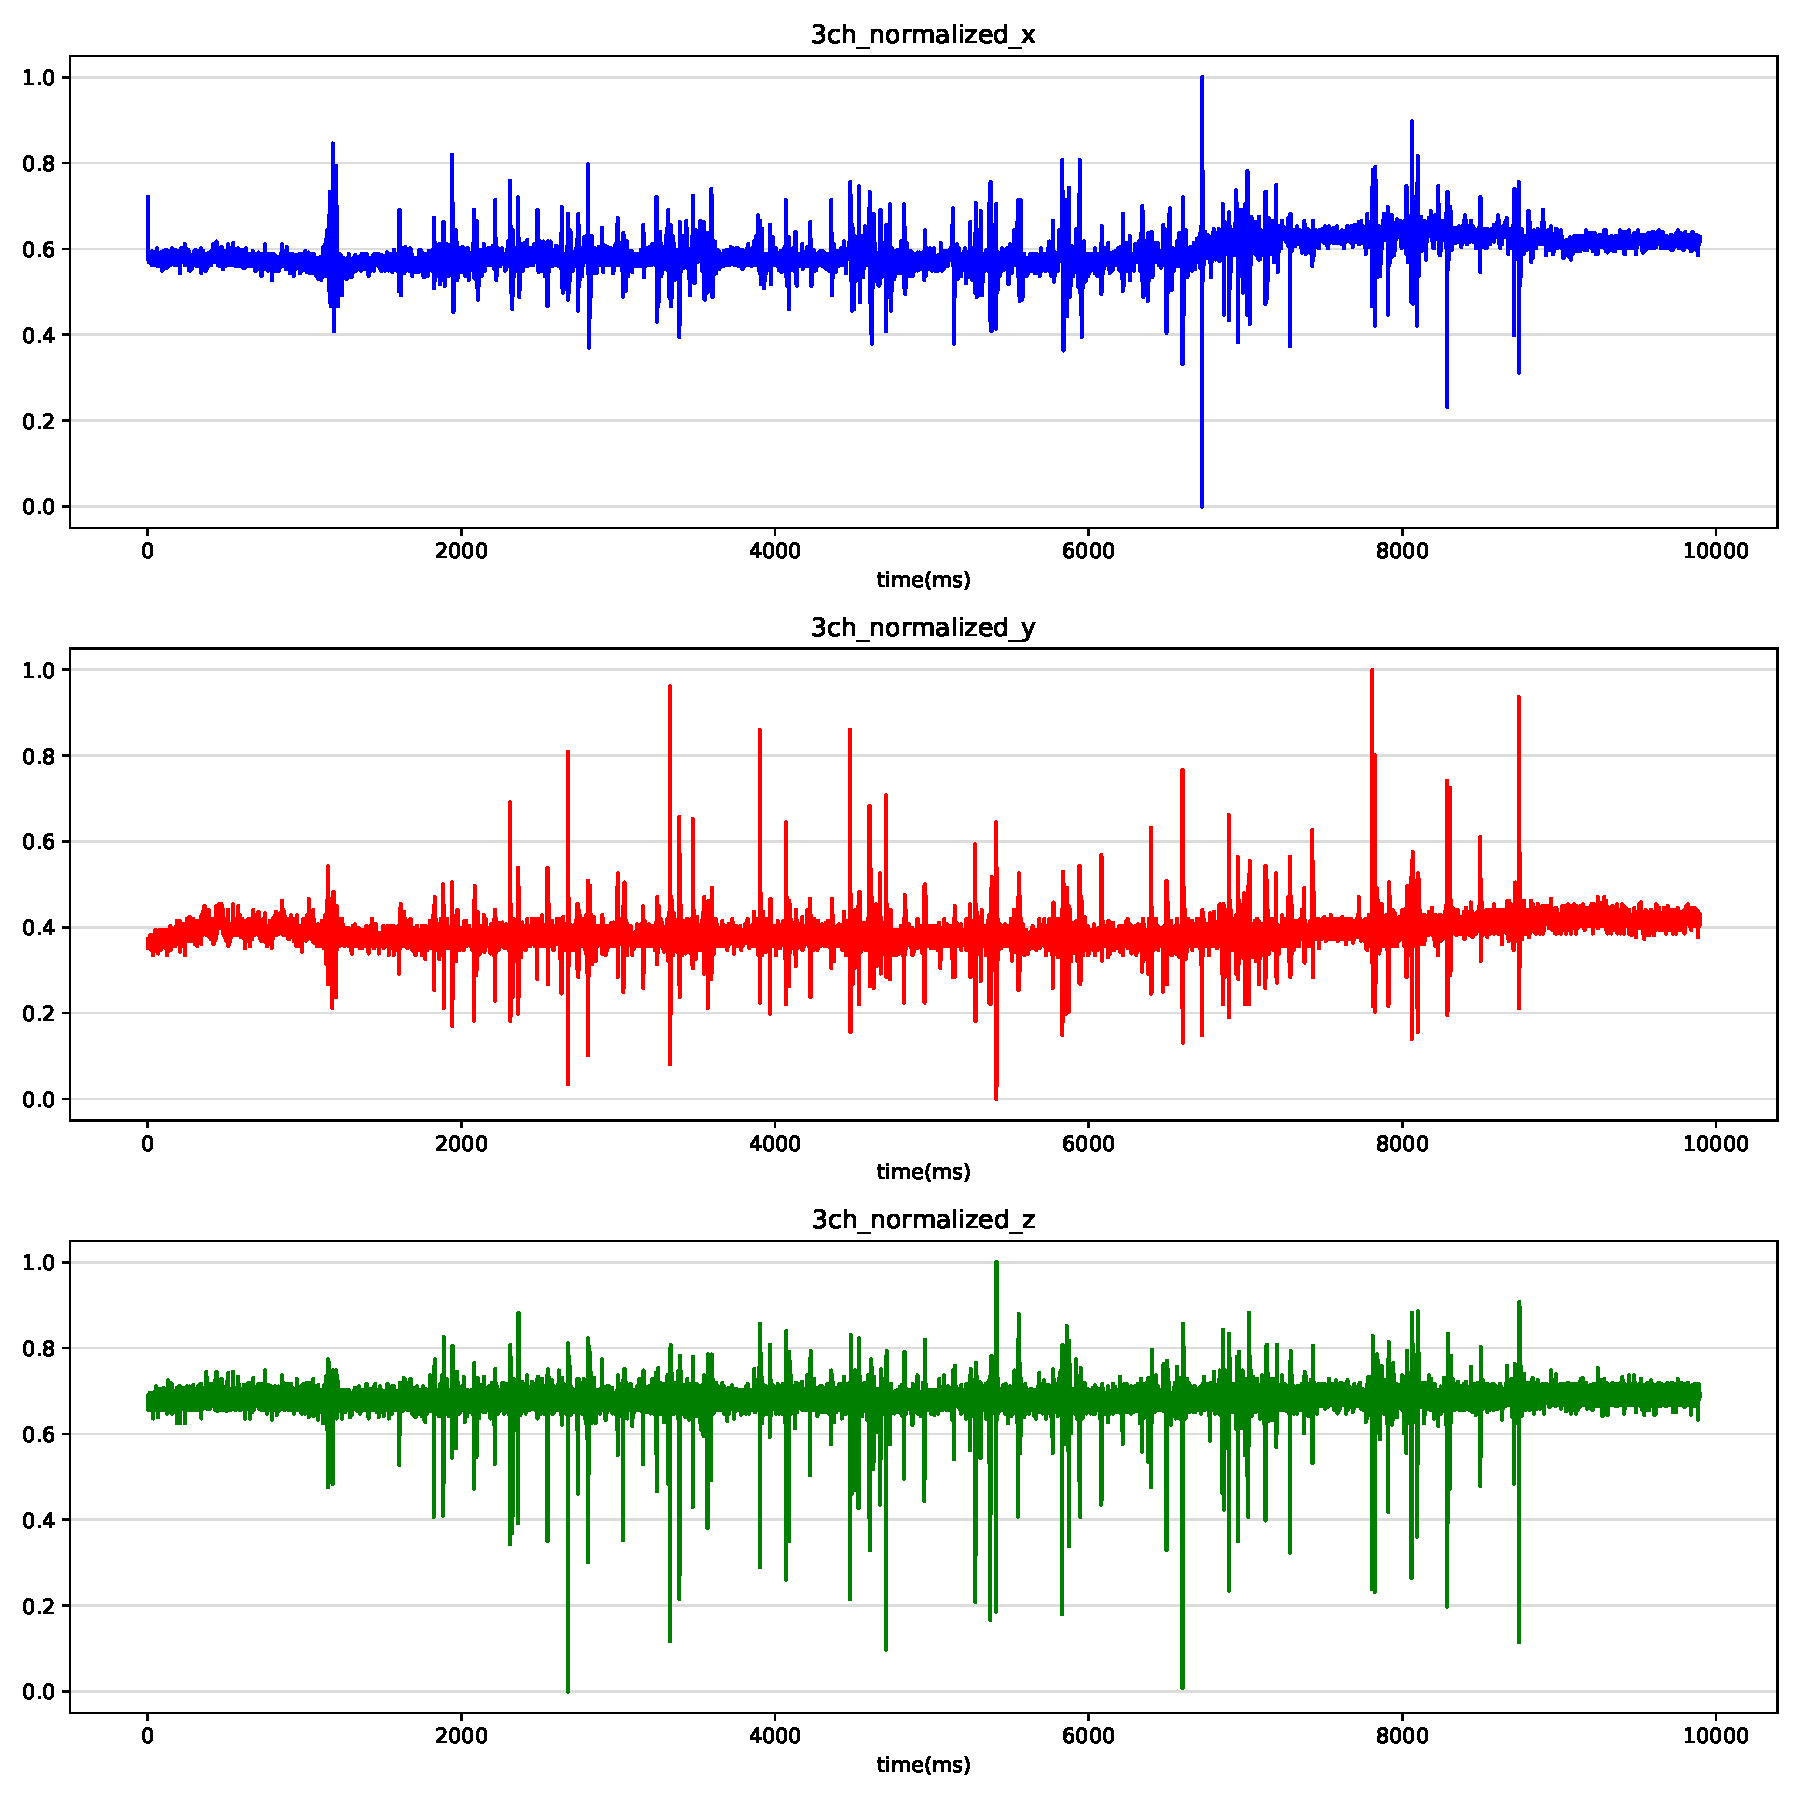
\includegraphics[width=12cm]{eps/3ch_normalized.pdf}
    \caption{Art Grass をなぞった際の3軸加速度データに正規化を適用した場合の出力信号例}
    \label{fig:normalize}
   \end{center}
   \end{figure}
   


\subsection{モデルの構成}
本研究で用いた次元削減信号の分類用 CNN のモデルの構成を以下の表\ref{tab:model_arc}に示す. 前処理にて次元削減を施した時系列加速度データは1次元信号であるので単純にデータ点数 * 1チャネルの入力層を用いる. 次元削減を施さない場合は3軸加速度データなので3チャネルの入力層を用いる. それ以降の構成は同じである. 
畳み込み層の活性化関数$f$として, ReLU関数を用いている. 
活性化関数は入力の総和をどのように発火させ後層に伝達させるかを司る関数である. 
ReLU 関数は負の値をノイズ値として扱う特徴があるが, 勾配消失の少なさと計算量削減の点で他の活性化関数よりも性能が良いとされ, 画像データの処理等で広く使用されている. 
本研究において, 入力の加速度データは負の値を持たないことから ReLU 関数を用いる. 
ReLU 関数は以下の式で定義される. 
\begin{equation}
    f(x)=\left\{\begin{array}{ll}x & (x>0) \\ 0 & (x \leq 0)\end{array}\right.
\end{equation}

\begin{figure}[H]
    \begin{center}
    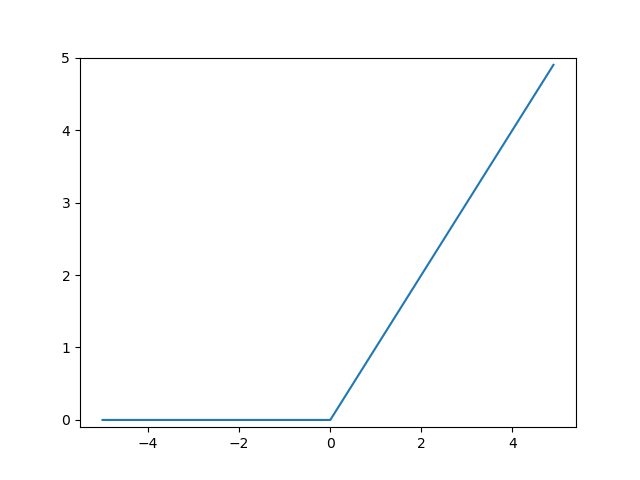
\includegraphics[width=12cm]{eps/relu.png}
    \caption{ReLU関数}
    \label{fig:relu}
   \end{center}
   \end{figure}
   
出力層の手前に全結合層を配置する. 全結合層の出力に活性化関数$f$をかけてモデル全体の出力とする. 
多クラス分類問題において, 出力層の活性化関数にソフトマックス関数を用いた計算が広く使用されている. ソフトマックス関数は以下の式で定義される. 
\begin{equation}
    y_{k}=\displaystyle\frac{\exp \left(a_{k}\right)}{\displaystyle\sum_{i=1}^{n} \exp \left(a_{i}\right)}
\end{equation}
ソフトマックス関数を用いることにより, 出力された値の総和を1に正規化し, ラベルに対する各々の値を確率として捉えることが容易になるという利点がある. 

\begin{table}[H]
\begin{center}
\caption{1次元分類用モデルの構成}
\begin{tabular}{|l||c c c c|c|}
\hline
layer\_name           & filters & kernel\_size & stride & activation & output\_map\_size \\ \hline \hline
input                 & -       & -            & -      & -          & 4096 * 1         \\ \hline
Conv1D\_1             & 64      & 5            & 1      & ReLU       & 4096 * 64          \\ 
Conv1D\_2             & 64      & 5            & 1      & ReLU       & 4096 * 64         \\ 
MaxPooling1D\_1       & -       & 2            & 2      & -          & 2048 * 64         \\ \hline
Conv1D\_3             & 128     & 5            & 1      & ReLU       & 2048 * 128        \\ 
MaxPooling1D\_2       & -       & 2            & 2      & -          & 1024 * 128        \\
Dropout\_1            & -       & -            & -      & -          & 1024 * 128        \\ \hline
Conv1D\_4             & 64      & 5            & 1      & ReLU       & 1024 * 64         \\ \hline
GlobalMaxPooling1D\_1 & -       & -            & -      & -          & 64                \\
Dropout\_2            & -       & -            & -      & -          & 64                \\ \hline
FullyConnected        & -       & -            & -      & Softmax    & 9                 \\ \hline
\end{tabular}
\label{tab:model_arc}
\end{center}
\end{table}

\section{評価指標}
本研究において, 評価実験で得られた出力に対して以下の4つの評価指標とそこから算出する重み付き平均を評価に用いる. 
また, それぞれの指標で用いる TP, TN, FP, FN を以下の表\ref{tab:def_conf}に示す. 

\begin{table}[H]
\begin{center}
\caption{TP, TN, FP, FNの定義}
\begin{tabular}{|c|c|c|c|}
\hline
\multicolumn{2}{|c|}{\multirow{2}{*}{}} & \multicolumn{2}{c|}{Actual}                     \\ \cline{3-4} 
\multicolumn{2}{|c|}{}                  & positive               & negative               \\ \hline
\multirow{2}{*}{predicted}  & positive  & True Positives ( TP )  & False Positives ( FP ) \\ \cline{2-4} 
                            & negative  & False Negatives ( FN ) & True Negatives ( TN )  \\ \hline
\end{tabular}
\label{tab:def_conf}
\end{center}
\end{table}

\begin{itemize}
  \item 精度( Accuracy )
 
  予測結果全体と, 正解ラベルの値がどれぐらい一致しているかを示す. 
  \begin{equation}
    {  Accuracy =\frac{T P+T N}{T P+F P+F N+T N}}
  \end{equation}
  \item 適合率 ( Precision )
  
  あるクラスにおいて, 予測されたもののうち, そのクラスの正解ラベルを有しているものの割合を示す. 
  \begin{equation}
     {  Precision =\frac{T P}{T P+F P}}
  \end{equation}
  \item 再現率 ( Recall )
  
   あるクラスにおいて, 正解ラベルを有しているものうち, 予測でそのクラスに分類されたものの割合を示す. 
  \begin{equation}
     {  Recall =\frac{T P}{T P+F N}}
  \end{equation}
  \item F値 ( $F-measure$ )
  
  トレードオフの関係にある適合率と再現率について両者の調和平均を示す. 
  \begin{equation}
     { F-measure =\frac{2 \cdot  Recall.Precision }{ Recall+Precision }}
  \end{equation}
\end{itemize}

上記の4つの評価指標は, 判別された各クラスに対して値が決まる. したがって9種のクラス分類を行う本研究ではモデルに対して評価指標が噴出し正確な評価につながらない事が考えられる. そこで重み付き平均を導入する. これは多クラスそれぞれのデータ件数の比率を重みとして上記4つのスコア平均を計算する. 
\begin{equation}
    {weighted  X =\frac{\sum w_{i} x_{i}}{\sum w_{i}}}
\end{equation}


% Local Variables:
% TeX-master: "main"
% mode: yatex
% End:



%#!platex --src-specials main.tex

\chapter{実験結果}
\label{chap:result}
本章では実験による結果を述べる. 
以下に各種次元削減を適用した1軸加速度触覚データと正規化を施した3軸加速度触覚データ, 無加工の3軸加速度触覚データを CNN で分類し, 出力から得られた4つの評価指標の値を以下の表\ref{tab:result}と図\ref{fig:accuracy}, \ref{fig:precision}, \ref{fig:recall}, \ref{fig:fmeasure}に示す. 

\begin{table}[htp]
\begin{center}
\caption{各データ処理手法に対する評価指標値}
\begin{tabular}{|c||c|c|c|c|}
\hline
data name           & accuracy & precision & recall & F-measure \\ \hline \hline
SA321-x             & 0.8571   & 0.8851    & 0.8571 & 0.8583    \\ \hline
SA321-y             & 0.8061   & 0.8384    & 0.8061 & 0.8020    \\ \hline
SA321-z             & 0.8163   & 0.7922    & 0.8163 & 0.7947    \\ \hline
SoC321              & 0.8367   & 0.8977    & 0.8367 & 0.8599    \\ \hline
Mag321              & 0.8673   & 0.9201    & 0.8673 & 0.8731    \\ \hline
PCA                 & 0.9184   & 0.9464    & 0.9184 & 0.9244    \\ \hline
DFT321              & 0.7653   & 0.9293    & 0.7653 & 0.8168    \\ \hline
original            & 0.9694   & 0.9767    & 0.9694 & 0.9694    \\ \hline
normalized original & 0.9184   & 0.9306    & 0.9184 & 0.9191    \\ \hline
\end{tabular}
\label{tab:result}
\end{center}
\end{table}

\begin{figure}[H]
    \begin{center}
    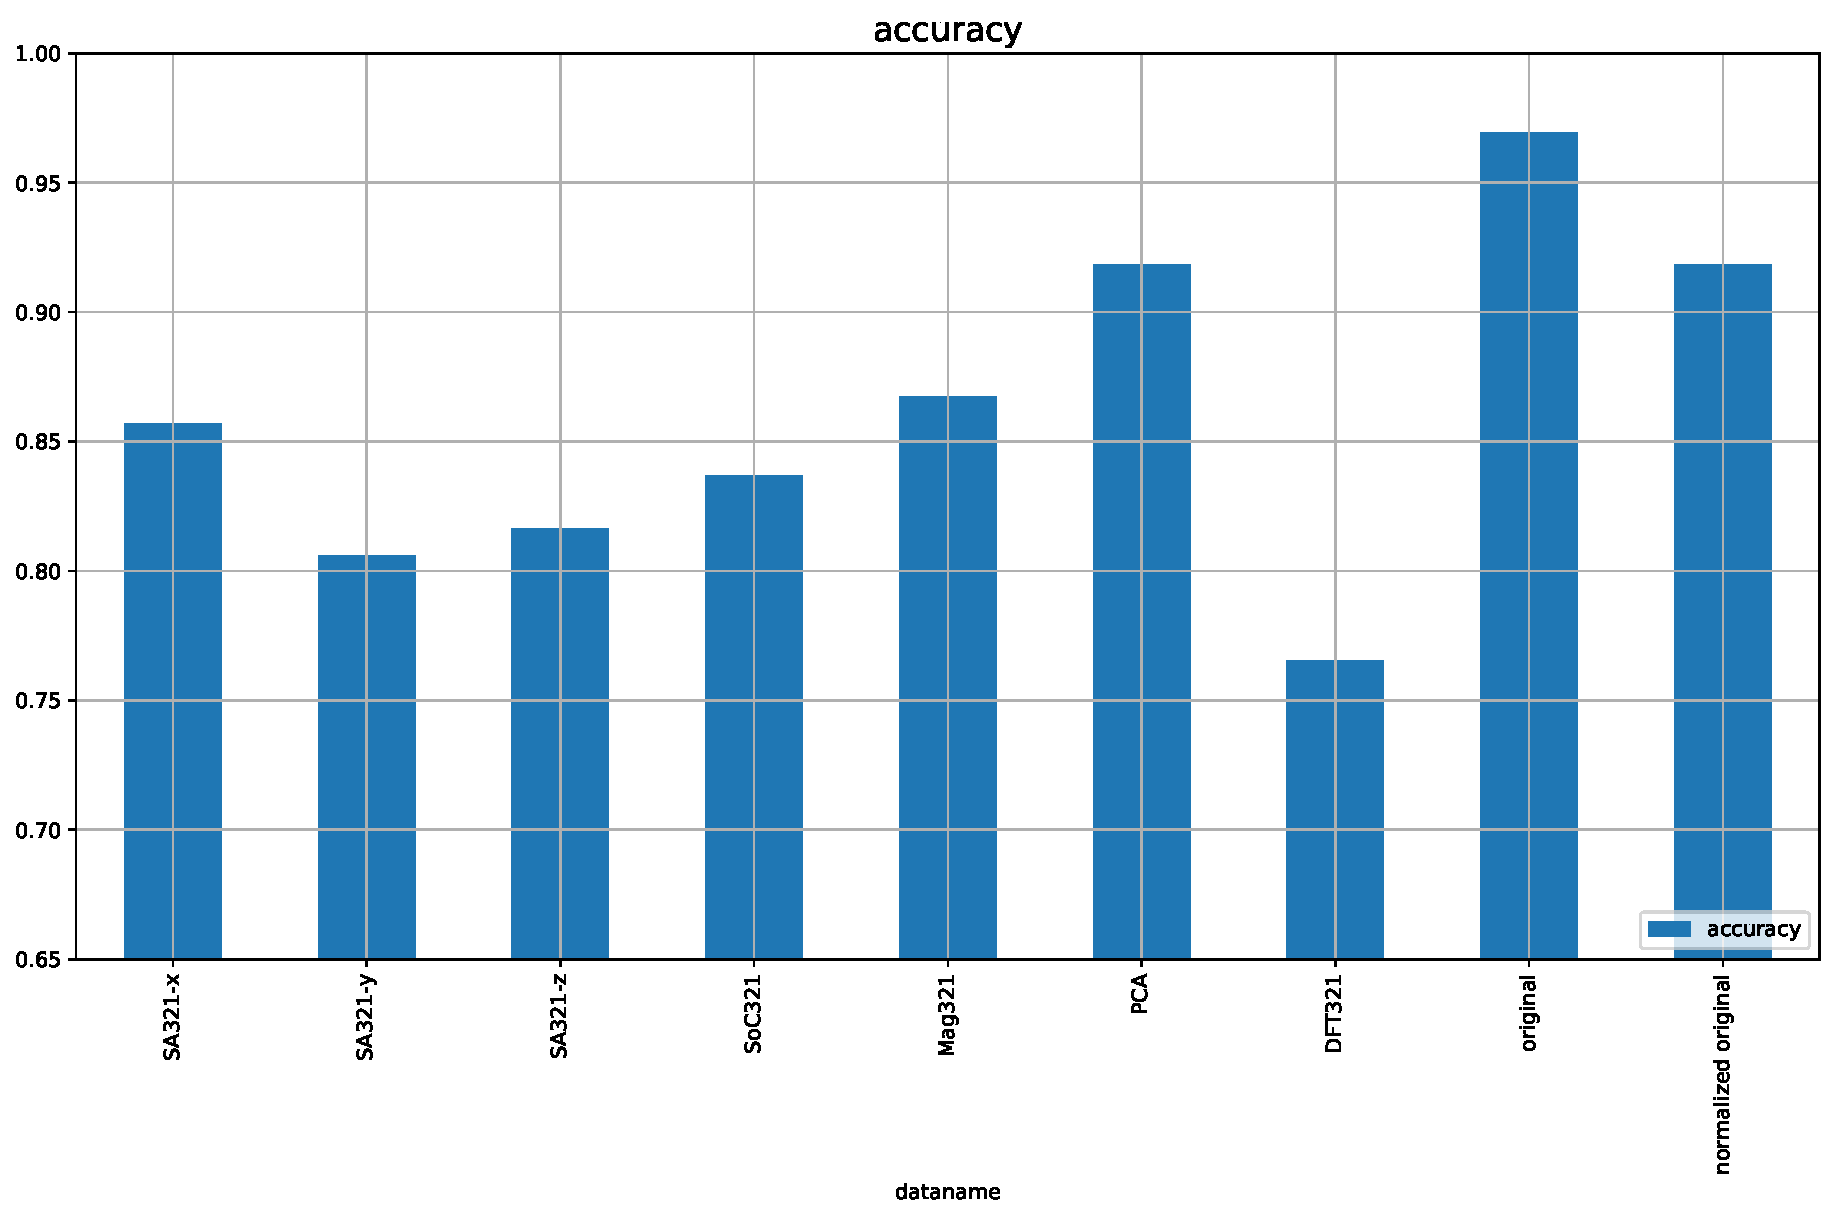
\includegraphics[width=12cm]{eps/accuracy.pdf}
    \caption{各データ処理手法に対する精度}
    \label{fig:accuracy}
   \end{center}
   \end{figure}
   
\begin{figure}[H]
    \begin{center}
    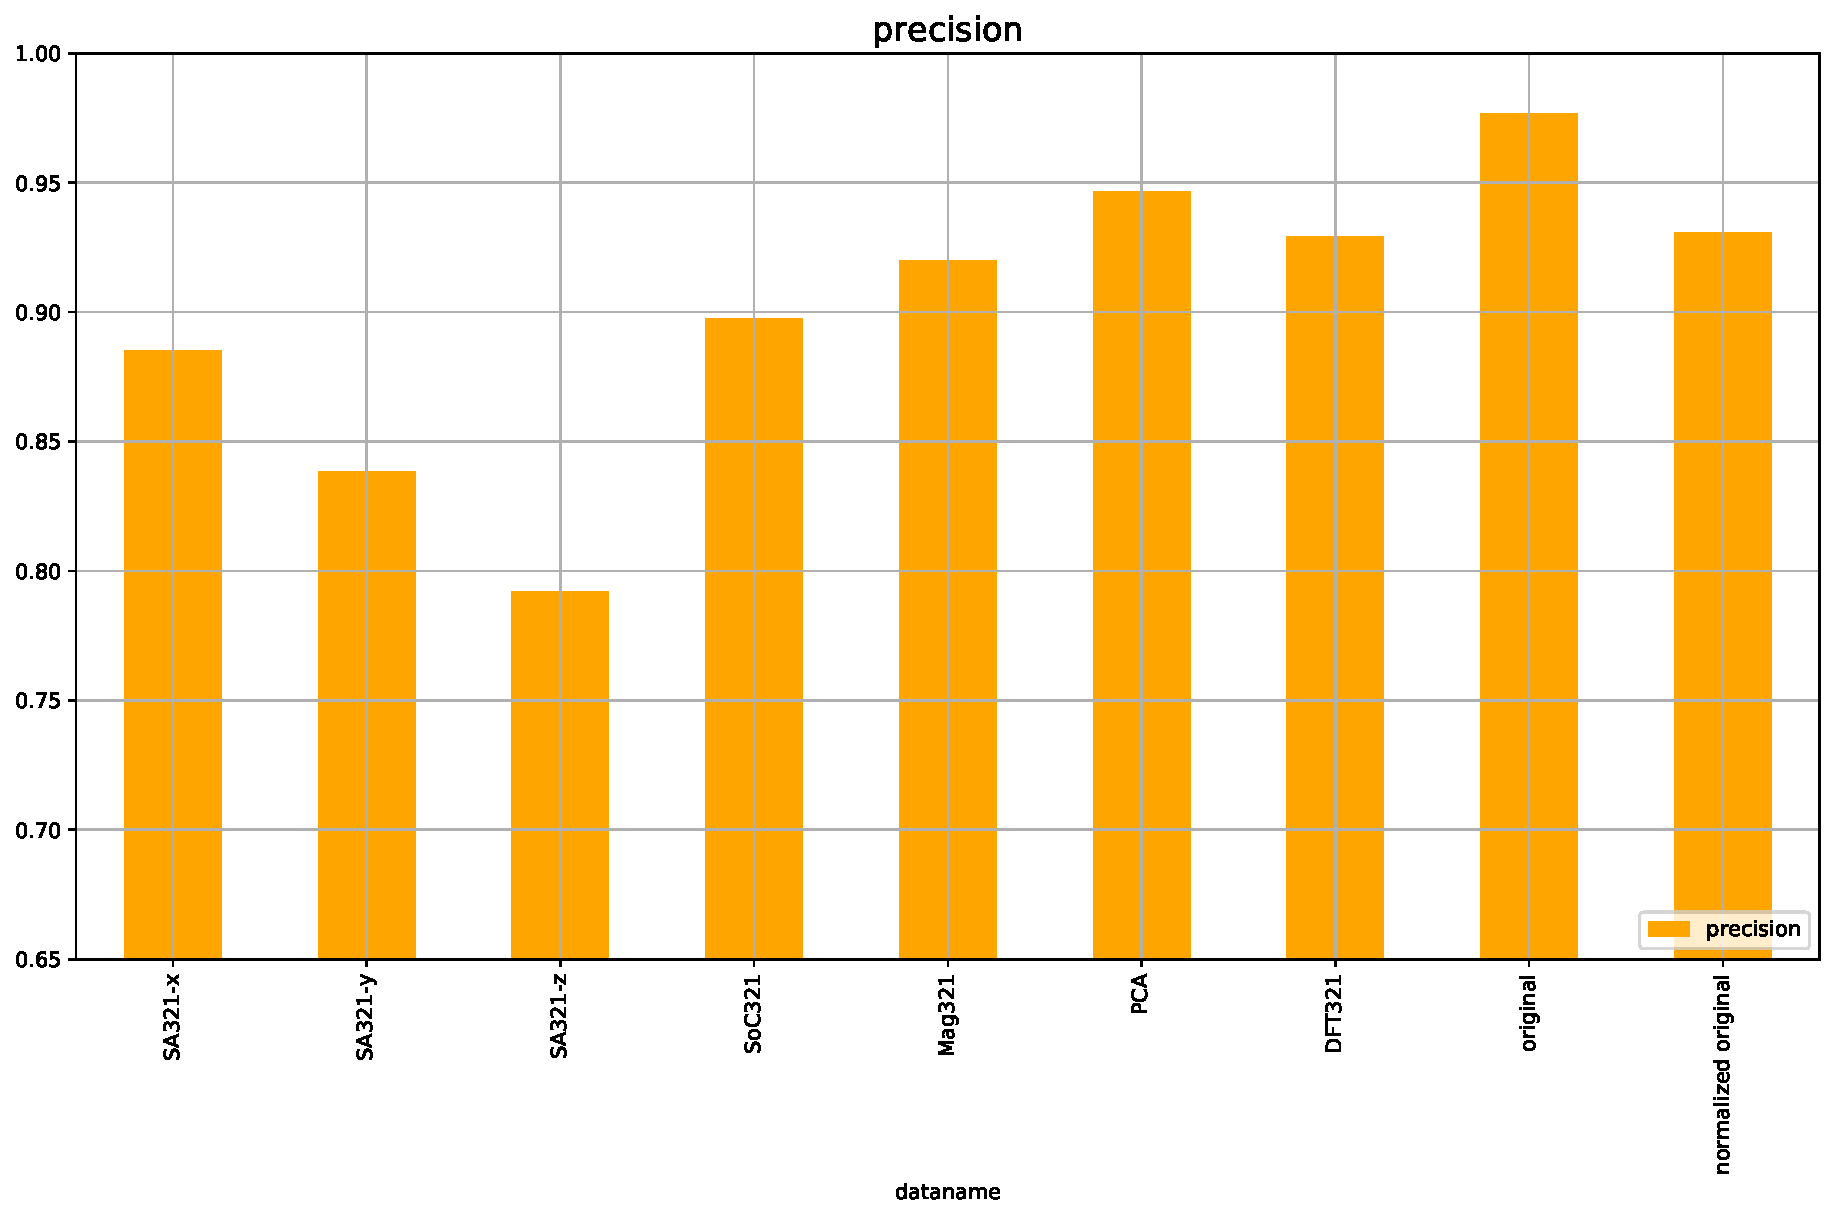
\includegraphics[width=12cm]{eps/precision.pdf}
    \caption{各データ処理手法に対する適合率}
    \label{fig:precision}
   \end{center}
   \end{figure}

\begin{figure}[H]
    \begin{center}
    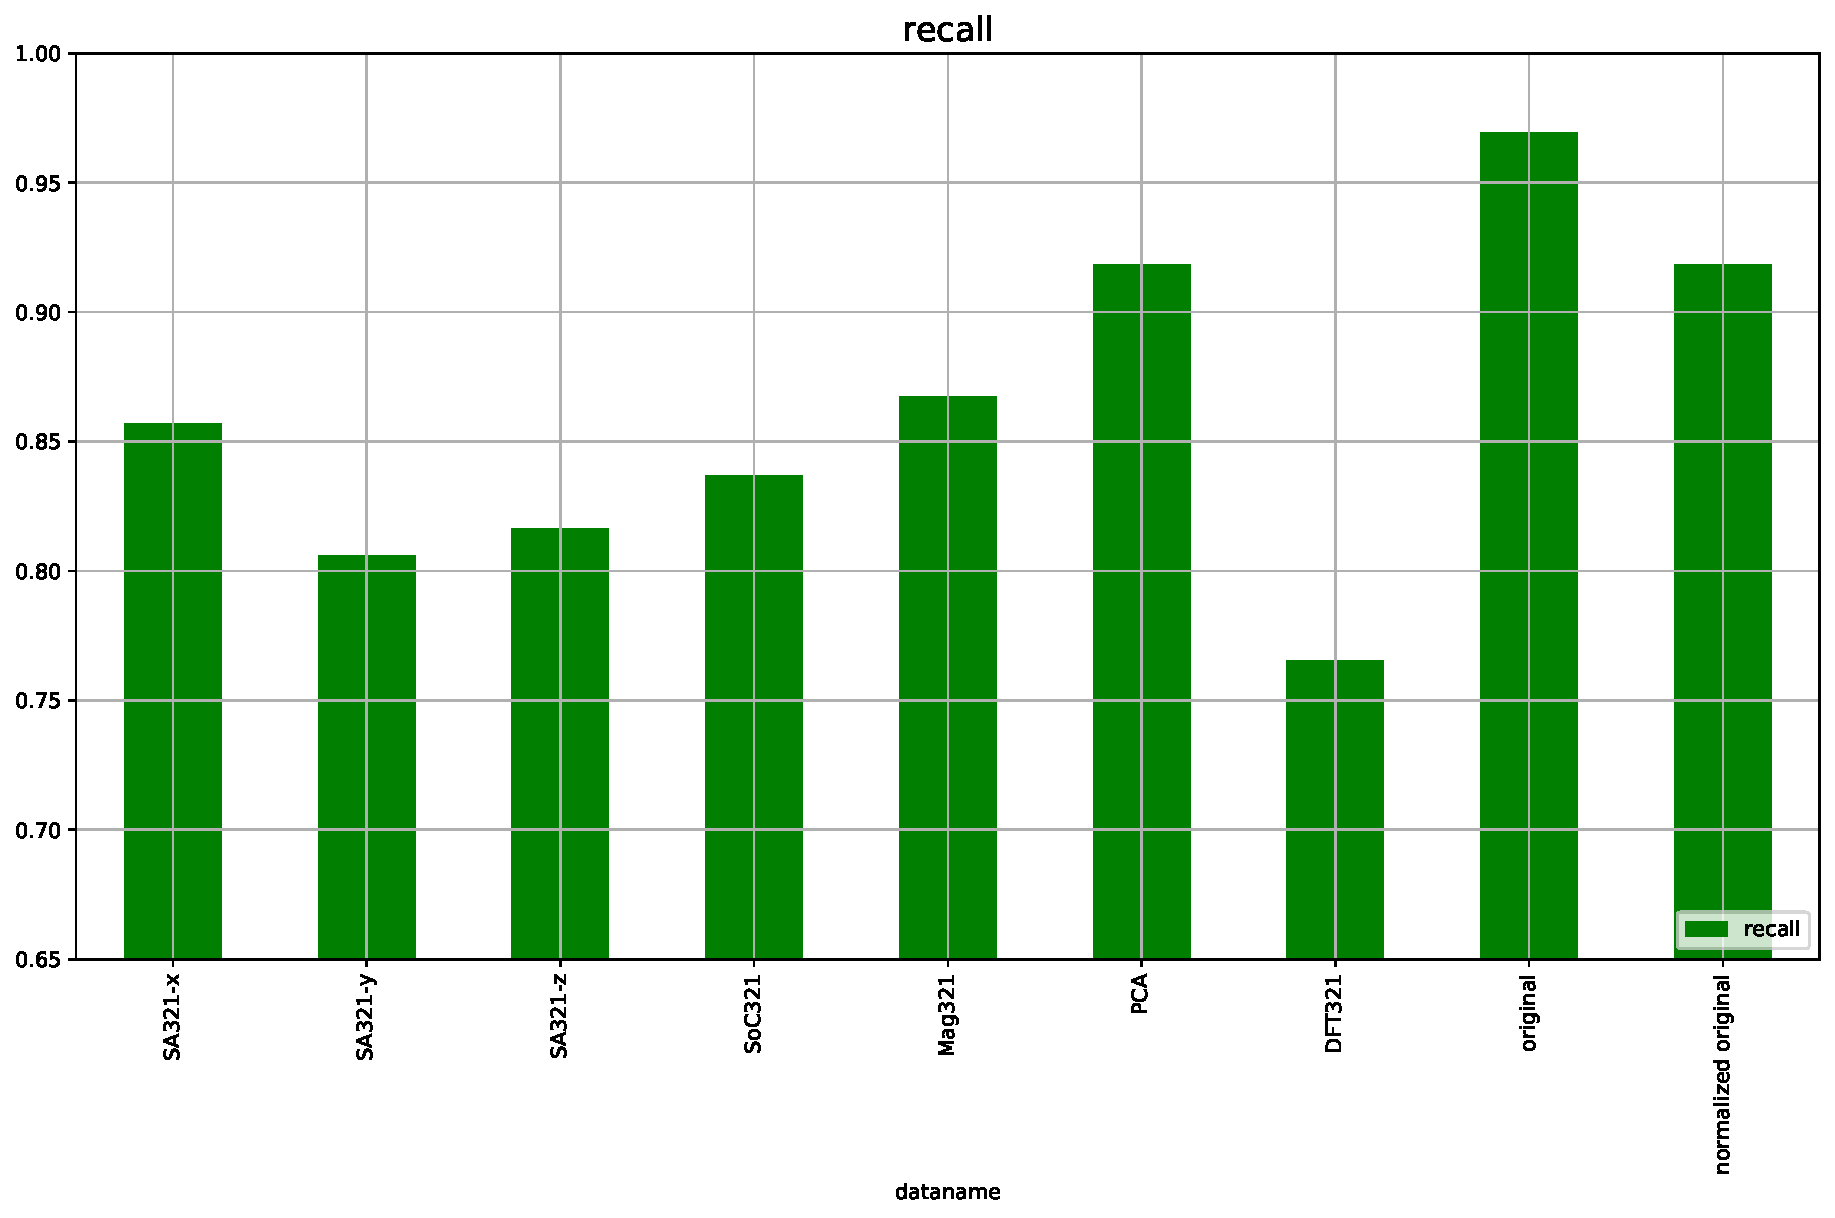
\includegraphics[width=12cm]{eps/recall.pdf}
    \caption{各データ処理手法に対する再現率}
    \label{fig:recall}
   \end{center}
   \end{figure}
   
\begin{figure}[H]
    \begin{center}
    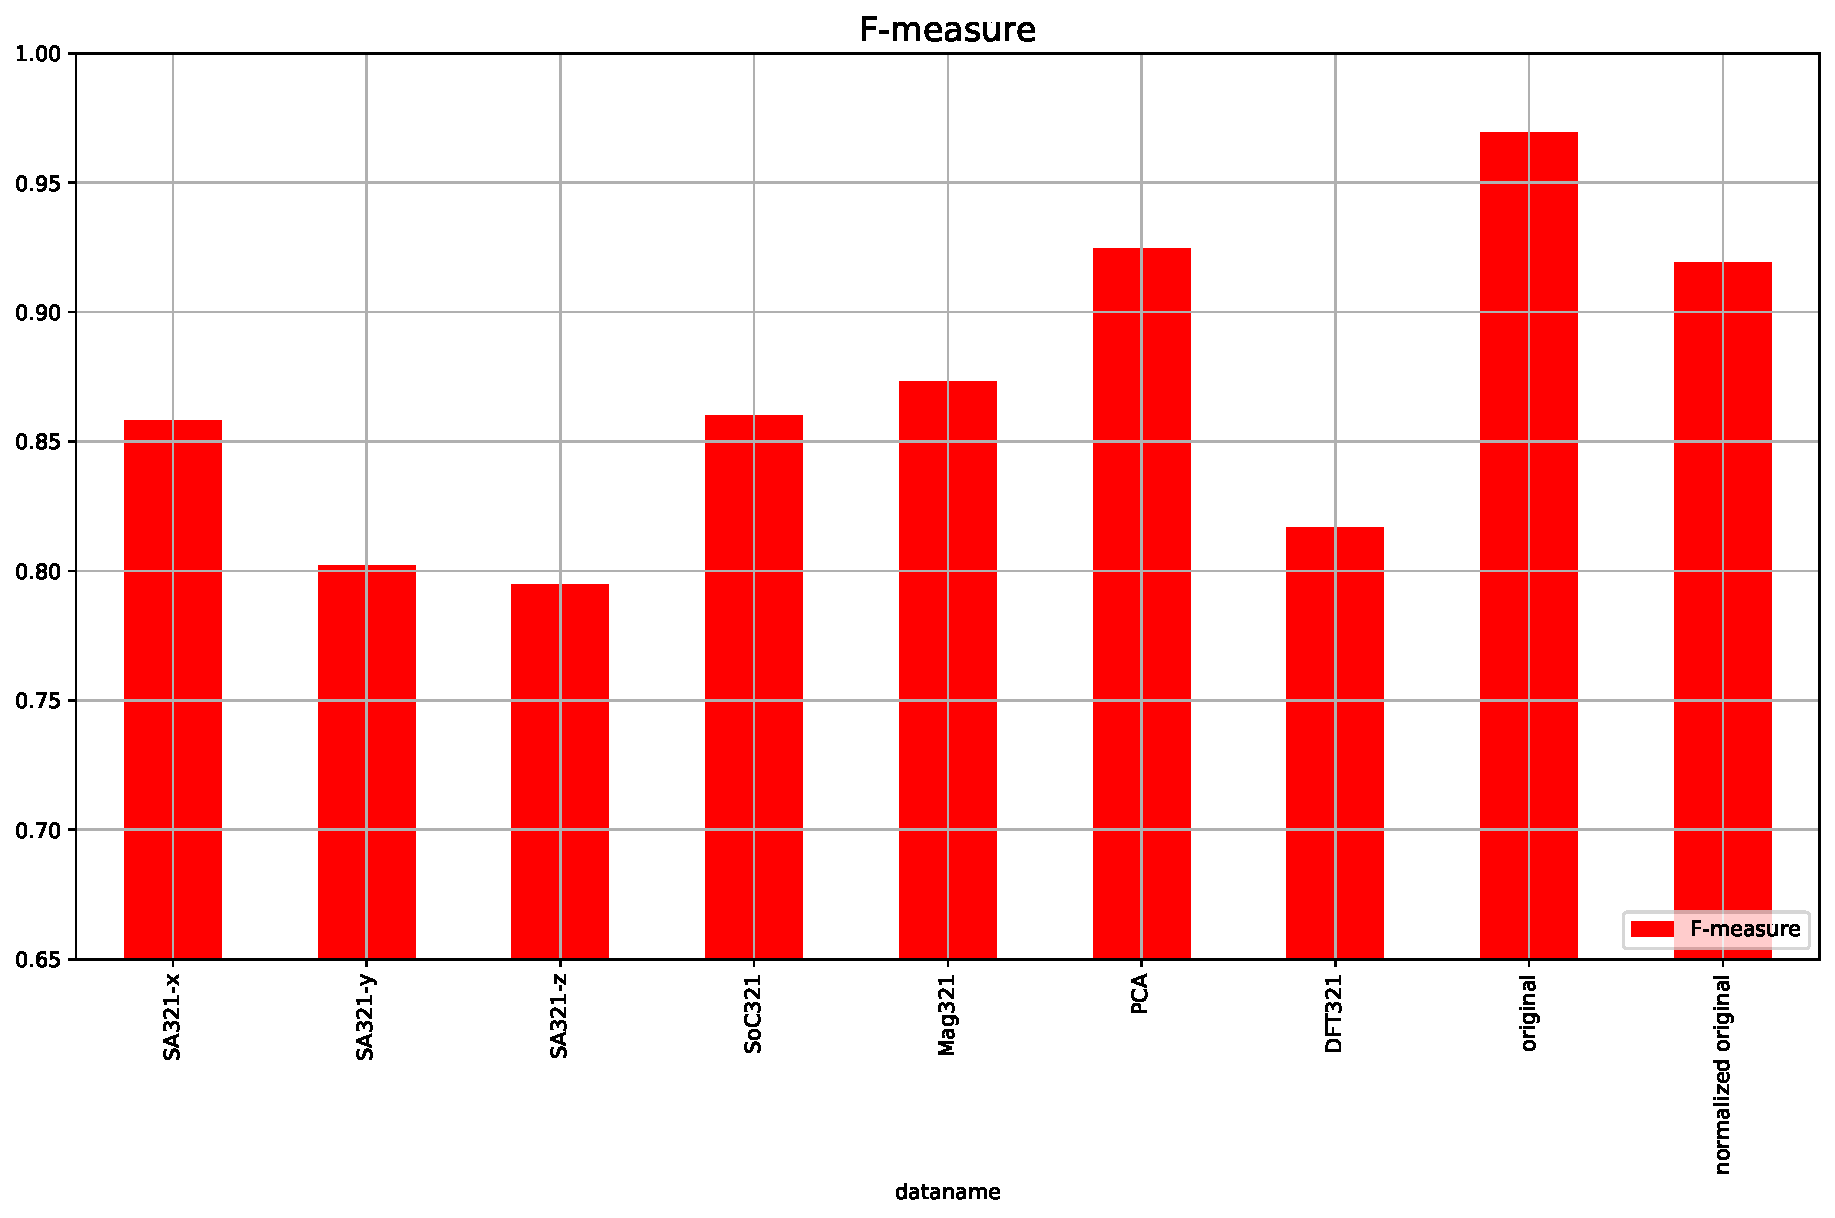
\includegraphics[width=12cm]{eps/F-measure.pdf}
    \caption{各データ処理手法に対するF値}
    \label{fig:fmeasure}
   \end{center}
   \end{figure}


% Local Variables:
% TeX-master: "main"
% mode: yatex
% End:


%#!platex --src-specials main.tex
\chapter{考察}
\label{chap:cons}
本章では実験結果に対する考察を述べる. 
\section{次元削減の有無による比較}
図\ref{fig:accuracy}, \ref{fig:precision}, \ref{fig:recall}, \ref{fig:fmeasure}より, 4つすべての評価指標において, 無加工の3軸加速度触覚データを入力に用いた場合の分類が最も高い値を記録している. 
特に精度において,  DFT321 で処理した触覚データの分類は76.5\%に比べ無加工の3軸加速度触覚データは96.9\%と20\%以上高い. 
また4つすべての指標において, 次点の高い値を示した手法よりも3\%程度かそれ以上の分類性能を有していることがわかる. 
これらから今回比較したいかなる次元削減手法も, CNN での分類において有意な情報が欠損してしまい, 精度に大きく影響すると言える. 
したがって, 分類精度の観点から見ると3軸加速度触覚データに対して CNN での分類を行う場合は得られた3軸加速度触覚データを次元削減せず入力として使用する手法が最も優れていると言える.

次元削減を行ったデータの中で比較を行うと, 無加工の1軸抽出を行うアルゴリズムである SA321 において軸ごとにばらつきがあるもののx軸を抽出する SA321-x が比較的良い値を記録している. これはテクスチャ分類の際に重要となる, 指でテクスチャをなぞる際の表面に対して鉛直方向の軸に比較的近い軸であった事が考えられる. 
また, DFT321 に関して, 精度, 再現率に関して他の手法に比べともに76.5\%と低い値であったが, 適合率に関しては92.9\%と比較的良い値を記録している. これは分類問題に対して, 予測したクラスが確実にそのクラスに分類される尺度である. これより DFT321 は複雑な前処理を施したため, テクスチャに対してより狭く顕著である特徴を中心に抽出, 学習してしまいその特徴に高いレベルで合致しなければ正しく分類ができないような現象が起きたことが推測される. 

また, 次元削減を行う主目的である計算量の削減に関して, それぞれのデータの前処理と学習にかかった時間を以下の図\ref{fig:process_time}に示す. 
図\ref{fig:process_time}より, 多少の差はあるが学習時間には有意差は無く, むしろ次元削減を施した PCA と DFT321 は明らかに無加工の3軸加速度データに比べ処理時間がかかっている. 
処理時間は使用するコンピュータ, ハードウェアにも大きく起因し単純な計算量の比較とは全く言えないが, 少なくとも CNN の学習に関して影響はほぼ与えないと考える. 

\begin{figure}[H]
    \begin{center}
    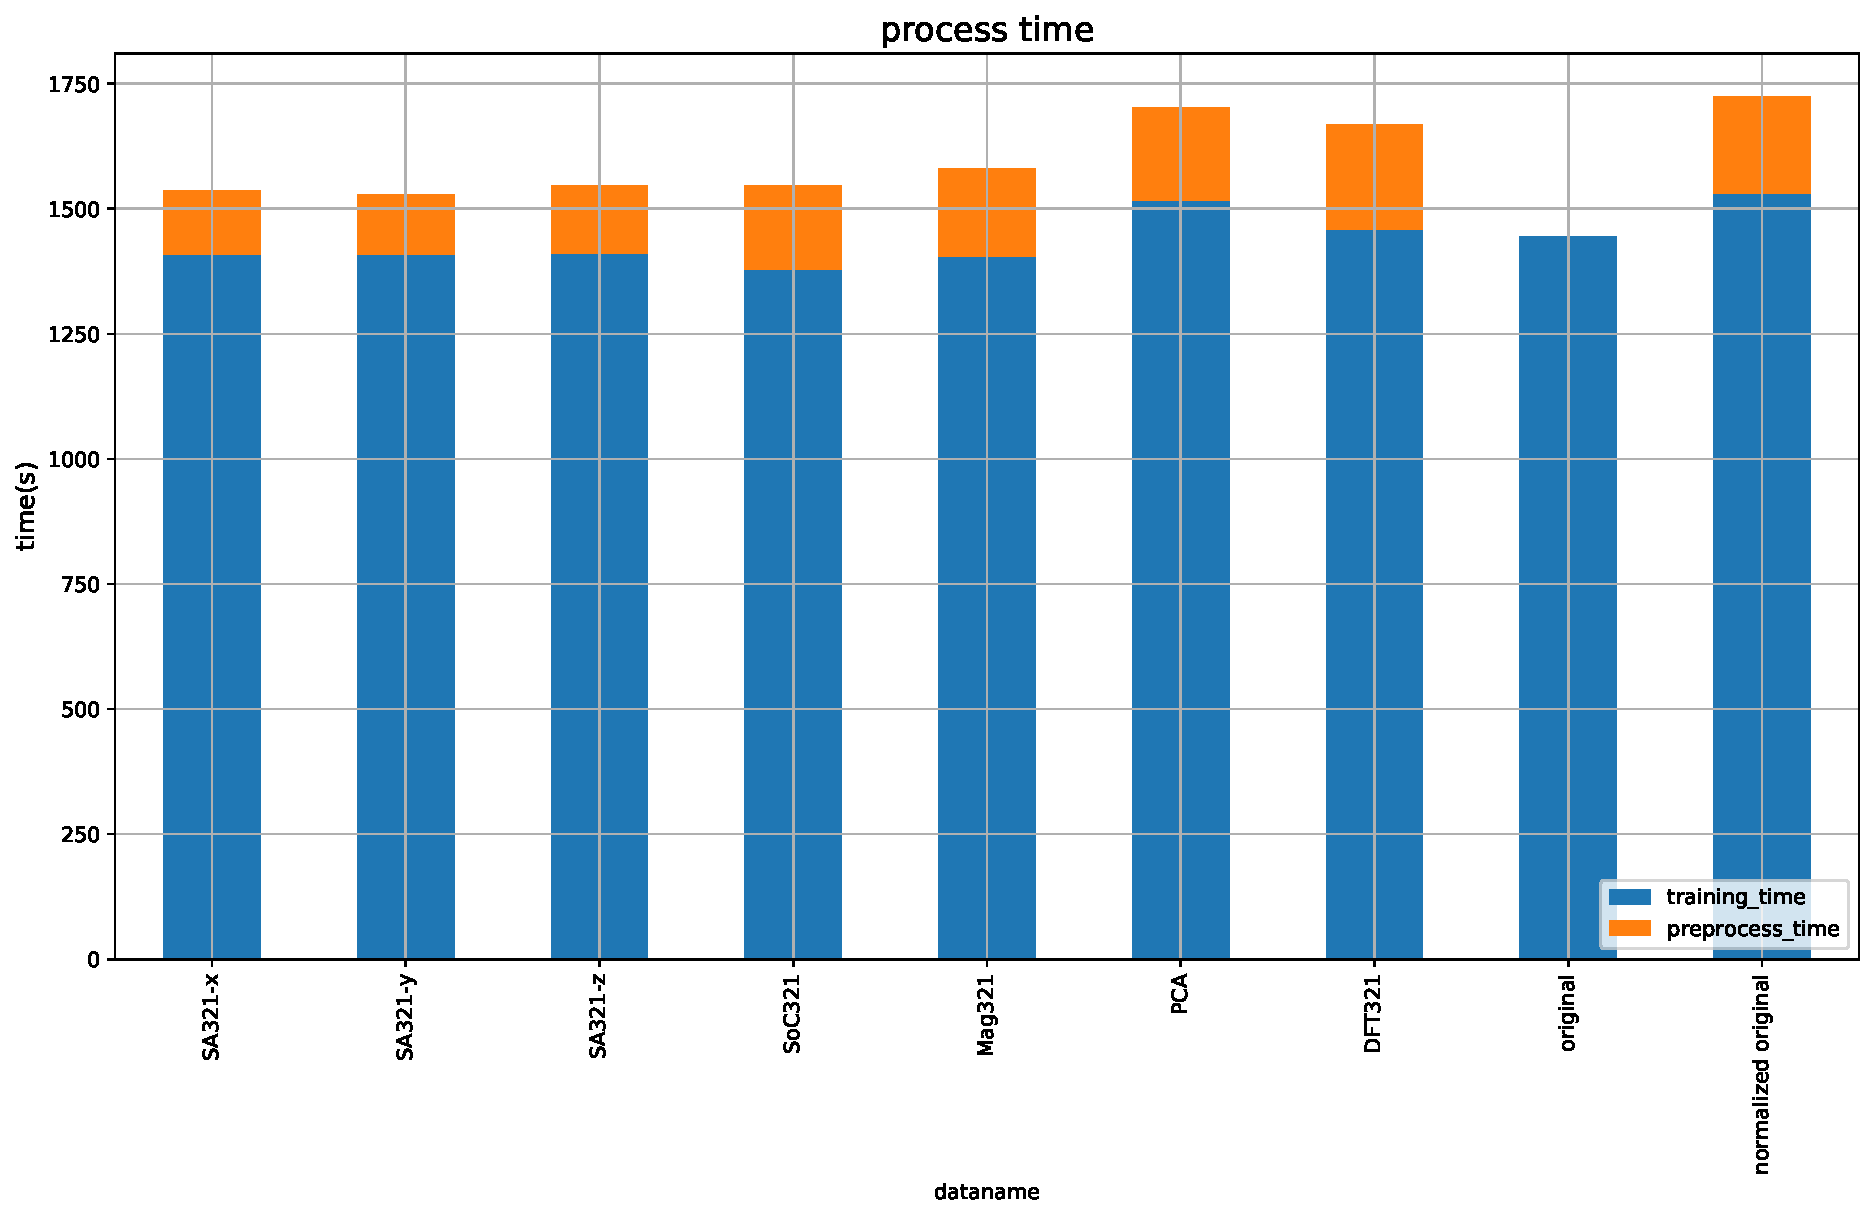
\includegraphics[width=12cm]{eps/process_time.pdf}
    \caption{各データ処理手法に対する前処理時間と学習時間}
    \label{fig:process_time}
   \end{center}
   \end{figure}
   
\section{正規化の有無による比較}
正規化の有無についても比較を行う. この比較に関しても4つすべての評価指標において, 無加工の3軸加速度触覚データを入力に用いた場合の分類が正規化を行った3軸加速度触覚データに比べ高い値を記録している. 
したがって, 分類精度の観点から見ると3軸加速度触覚データに対して CNN での分類を行う場合は得られた3軸加速度触覚データの正規化は有意ではないと言える.
正規化が分類に有利に働かなかった理由として, 3軸加速度のスケールがほぼ同じであることに起因すると考える. 
正規化はパラメータ間のスケールを統一しネットワークのパラメータによる更新幅の違いを吸収する役割を持つ. 
しかし3軸加速度データに関しては同一センサから得た3軸を3つのパラメータとして取り扱うのでスケールはほぼ同一な上, そこに付随するスケーリング前の値がクラス分類に有意な特徴となったと思われる. 
したがって正規化を行った際に特徴が一部消失し, 無加工の3軸加速度触覚データよりも低い分類精度を記録したと考える. 
% Local Variables:
% TeX-master: "main"
% mode: yatex
% End:


%#!platex --src-specials main.tex
\chapter{おわりに}
\label{chap:conc}
本研究では, 3軸加速度触覚情報をもとに次元削減などの信号処理をおこなった情報を用いた機械学習で分類し, 分類精度に対する4つの評価指標を用いて触覚情報における3軸加速度情報の取扱いについて検討を行った. 
評価実験の結果, 3軸加速度の触覚情報が得られ, かつ分類の精度を重要視した処理を行う場合, 何も処理を行わない3軸加速度の触覚情報が次元削減や正規化を行った3軸加速度の触覚情報に比べ有用であると結論付けた. 今後の課題として, 分類精度の観点だけではなく厳密な計算量の観点も含めた検討を行い, テクスチャの再現や提示を行うシステムに用いた場合にどのような影響を及ぼすか考察が求められると考える.


% Local Variables:
% TeX-master: "main"
% mode: yatex
% End:



%謝辞
%#!platex --src-specials main.tex

\begin{thanks}
本研究を実施するにあたり,研究の方向性や実施並びに論文執筆に関しての多くの助言を頂き熱心に指導していただいた熊本大学大学院先端科学研究部 情報・エネルギー部門 医用福祉工学分野 准教授 嵯峨 智先生に心から感謝いたします. また, 本研究において研究内容に様々な助言をくださり, 実験用のデータの提供やプログラムの助言などを頂いた筑波大学大学院 システム情報工学研究科 コンピュータサイエンス専攻 博士後期課程 2 年 富田洋文さん, 博士前期課程 2 年 我妻 正太郎さん, 熊本大学大学院自然科学教育部 情報電気工学専攻 情報工学教育プログラム 博士前期課程 2 年 黒木詢也さんに深く感謝いたします. 
本研究において日頃より応援していただいた熊本大学大学院自然科学教育部 情報電気工学専攻 情報工学教育プログラム 博士前期課程 1年 池田尚登さん, 石丸嵩也さんに感謝いたします.
\end{thanks}
% Local Variables:
% TeX-master: "main"
% mode: yatex
% End:



% 参考文献
%\include{cite}
\bibliographystyle{junsrt}
\bibliography{ref}


%\include{huroku}




\end{document}

% Local Variables:
% TeX-master: t
% mode: yatex
% End:

% \documentclass[dvipdfmx,autodetect-engine]{jsarticle}
% \usepackage{tikz}

% \title{サンプル文書}
% \author{著者}

% \begin{document}
% \maketitle

% \begin{abstract}
% 日本語を用いた文書を作成します。    
% \end{abstract}

% \section{はじめに}

% TikZ図版もテストします。

% \begin{center}
% \begin{tikzpicture}
% \node[draw,fill=red!20!white,circle] (S) at (0,0) {はじめ};
% \node[draw,fill=blue!20!white,circle] (G) at (2,2) {おわり};
% \draw[very thick,->] (S) -- (G);
% \end{tikzpicture}
% \end{center}

% \end{document}
